\section{Non-LArTPC Instruments}\label{sec:FTBF}
The Fermilab Test Beam Facility (FTBF) receives a 120~GeV$/c$ primary proton beam with variable intensity, split by electrostatic septa from beam circulating in the Main Injector. Each supercycle of the Fermilab accelerator complex, roughly 60 seconds in duration, includes a four-second "spill" of primary beam to FTBF. Primary beam is sent to either or both of two experimental halls, named Meson Test and Meson Center.  

The LArIAT experiment utilized the Meson Center beam line and had this primary beam focused onto a tungsten target. The resulting secondary charged particle beam is selected to have peak momentum between 8-80\,GeV$/c$ and is transported to the LArIAT experimental hall, designated MC7, where it is focused onto a copper target. This target, and the steel collimator hosting it, form the beginning of the tertiary particle beam and the LArIAT apparatus shown in  Fig.~\ref{fig:tert-layout}.  For most of the LArIAT data taking this secondary beam peak momentum was fixed at 64~GeV$/c$, although some lower secondary beam momentum settings were explored.  With such an energetic secondary beam on it, the copper target produces a tertiary beam which is comprised of mostly pions and protons with a small fraction of electrons, muons, and kaons present as well. 

%%%%%%%%%%%%%%%%%%%%%%%%%%%%%%%%%%%%%%%%%%%%%%%%%%%%%%%%%%%%
\subsection{LArIAT Tertiary Beam}\label{sec:TertiaryBeam}
%%%%%%%%%%%%%%%%%%%%%%%%%%%%%%%%%%%%%%%%%%%%%%%%%%%%%%%%%%%%

The tertiary beam consists of a target and collimator system and two bending magnets in a similar configuration used for the  MINERvA T-977 test beam calibration~\cite{MinervaTestbeam}. A set of four wire chambers and two time-of-flight scintillating paddles, also shown in Fig.~\ref{fig:tert-layout}, provide tracking, momentum determination, and particle identification (PID). 

The geometry of the tertiary beam line in MC7 has been optimized for LArIAT.  A $13^\circ$ production angle at the target and its enclosing collimator, as well as a $10^\circ$ bend through a pair of dipole magnets provide particle momenta spectra tunable in the range from 0.2 to 2.0~GeV/c, as a function of the field intensity in the magnets.

\begin{figure}[!h]
\begin{centering}
\vspace{-0.3cm}
\includegraphics[height=5.3in]{figures/LArIATBeamline.png}
\caption{
{\scriptsize \sf The tertiary beam line layout. Upstream and downstream collimators are in gray, bending magnets in yellow, wire chambers are in red, and the liquid argon TPC volume in green.}
}
\label{fig:tert-layout}
\end{centering}
\end{figure}

In the subsequent sections, we will detail the various subsystems installed along the beamline

%%%%%%%%%%%%%%%%%%%%%%%%%%%%%%%%%%%%%%%%%%%%%%%%%%%%%%%%%%%%
\subsubsection{Time-of-Flight System}\label{sec:TOF}
%%%%%%%%%%%%%%%%%%%%%%%%%%%%%%%%%%%%%%%%%%%%%%%%%%%%%%%%%%%%

The LArIAT time-of-flight (TOF) detector system consists broadly consists of two scintillator paddles, which bracket the beamline and are shown in blue in Figure~\ref{fig:tert-layout}. The exact details of the of the TOF system were changed between Run-II and Run-III to allow for better performance and timing resolution.

\paragraph{\textbf{TOF System for Run-I and Run-II:}}
The upstream paddle, shown in Figure \ref{}, has a relatively small active area (10~cm x 6~cm ) and was chosen to be a relatively thin piece of scintillator to minimize any impact on the momentum of the particles coming from the target. Light guides were mounted on all four edges which lead to two \textit{insert PMT type} PMTs mounted on the beam left side. The downstream paddle, shown in Figure \ref{fig:TOFSystemRunIandII}, was chosen to have a slightly larger area (14~cm x 14~cm) and had two \textit{insert PMT type} PMTs which were read out on opposite ends of the paddle.

\begin{figure}[!h]
\begin{centering}
\vspace{-0.3cm}
%\includegraphics[height=2.3in]{figures/tofdelay.png}
\caption{
{\scriptsize \sf Pictures of the TOF system as was deployed during Run-I and Run-II data taking. The left image is of the upstream TOF paddle and the right image is of the downstream TOF paddle }
}
\label{fig:TOFSystemRunIandII}
\end{centering}
\end{figure}

\paragraph{\textbf{TOF System for Run-III:}}
Two modifications were made to the downstream TOF paddle for Run-III to improve the efficiency and timing of the system. The large area scintillator paddle was replaced with a slightly smaller paddle more similar to the upstream and was now readout with four new PMT's (2" Hamamatsu PMTs (R-1828) inherited from the muon g-2 experiment(E821) at BNL) located on the diagonals of the counter, as shown in Figure \ref{fig:TOFSystemRunIII}.

\begin{figure}[!h]
\begin{centering}
\vspace{-0.3cm}
\includegraphics[height=2.3in]{figures/TOFRunIII.png}
\caption{
{\scriptsize \sf Image of the modified downstream TOF system deployed during Run-III data taking }
}
\label{fig:TOFSystemRunIII}
\end{centering}
\end{figure}


%The active area of the upstream paddle is relatively small ( 10~cm x 6~cm ) and that of the downstream paddle is somewhat larger ( 14~cmx 14~cm ). Lightguides are mounted on all four edges of each paddle. In the first two LARIAT production runs, each of the paddles was read out by two (xxkxkxkxk) photomultiplier tubes (PMTs), The long axis of the downstream paddle was directed horizontally and read out at either end. The upstream paddle was rotated by 45 degrees with respect to the horizontal and its two PMTs were mounted to the left side. In run 3, four more PMTs were added to the system. The upstream paddle was read out with the original set of PMTs and the downstream paddle with four 2" Hamamatsu PMTs (R-1828) inherited from the muon g-2 experiment(E821) at BNL.

During data-taking cycles, signals from the TOF PMTs were sampled at 1 GHz
with a CAEN 1751 digitizer and 12 bit samples were stored in a circular memory buffer. In response to an experimental trigger, a 28.7 $\mu$ second window of samples, starting approximately 8.4 $\mu$sec before the trigger, was written to the
output. The amplitude of the TOF signals was typically 200 mV in the upstream TOF PMTs but only 50 mV in those of the downstream counter. The signals have a rise time (10-90\%) of 4 ns and a full width, half-maximum of 9 ns. The rate in the upstream counter was typically 15 kHz and much less, 400 Hz in the downstream counter.

Because the shape of signals from each TOF PMT was highly uniform, the time of the pulses was determined using an oversampled template derived from the data itself. The DC offset (pulse pedestal) is taken from samples far from the pulse, The template is stretched vertically to match the pedestal-subtracted pulse amplitude and moved horizontally to match the time. The pulse time-pickoff resolution is better than 100 ps and relative amplitude resolution is better than x\%. Since the average rate of pulses incident on the ToF system is modest, pulse pile up is not a significant problem. Given the uniform width of the pulses produced by any given PMT (sigma of 400 ps), the pulse width can be used to flag events where two pulses overlap closely in time. Simulations indicate that for pulses as close as 4 ns, a well-chosen pulse width cut is 90\% efficient.

To determine the particles' time of arrival, pulse times from the multiple PMTs mounted on each paddle had to be combined. During Run-I and II, with two PMTs mounted on each paddle, a simple average was used. In the case of the downstream paddle, with PMTs mounted at opposite ends, the average corrected for the fact that transit time to the two PMTs depended on the particle's point of impact on the scintillator. A plot of the time of arrival {\it difference} between the two downstream PMTs vs the longitudinal impact point, made with the help of track stubs from the wire chamber system, is shown in Fig.~\ref{fig:tofdelay}. As expected, the time difference
changes systematically across the face of the scintillator.

\begin{figure}[!h]
\begin{centering}
\vspace{-0.3cm}
%\includegraphics[height=2.3in]{figures/tofdelay.png}
\caption{
{\scriptsize \sf $\Delta-t$ between times registered on two downstream paddles.}
}
\label{fig:tofdelay}
\end{centering}
\end{figure}

Taking the average minimizes ToF errors arising from optical path differences in the scintillator, However, even for a set of particles which pass through a single small area of the paddle, the times of pulses registered in the two PMTs are still spread by approximately 300~ps, an uncertainty which is probably caused by transit time jitter in the PMTs themselves. This jitter is evident in both the upstream and downstream detectors.

Although climate-control in the LArIAT experiment hall is fairly primitive, there is little sign of systematic timing drift over longer periods. The average time differences between pairs of PMTs reading out the same scintillator varied by no more than 150~ps over the 3-4 months of a data-taking period.

Finally, the amplitude of the ToF pulses (peak minus pedestal) reflects the energy deposited in the scintillator, largely through ionization.  At a given momentum, more massive particles such deuterons, protons, and kaons, will deposit more energy than less massive particles, such as electrons, muons, and pions. As described below, ToF and momentum information from the wire chambers can be combined to determine the particle's mass and hence its identity. Although the energy deposited in the scintillator isn't used to distinguish among the various particle types, it's clear from Figure~\ref{fig:tofamplitude} that the spectra of energy deposition for
electrons, pions, and protons are very different.

\begin{figure}[!h]
\begin{centering}
\vspace{-0.3cm}
%\includegraphics[height=2.3in]{figures/tofamplitude.png}
\caption{
{\scriptsize \sf Average upstream ToF pulse amplitude for protons and pions/positrons.}
}
\label{fig:tofamplitude}
\end{centering}
\end{figure}

%%%%%%%%%%%%%%%%%%%%%%%%%%%%%%%%%%%%%%%%%%%%%%%%%%%%%%%%%%%%
\subsubsection{Bending Magnets}\label{sec:Magnets}
%%%%%%%%%%%%%%%%%%%%%%%%%%%%%%%%%%%%%%%%%%%%%%%%%%%%%%%%%%%%
The pair of spectrometer magnets in the LArIAT tertiary beam are Fermilab type "NDB" electromagnets, originally used in the anti-proton ring. These magnets provide the necessary bend in the particle trajectory to allow for a momentum measurement to be performed.  The magnets have a gap height of 14.224~cm, a gap width of 31.75~cm, and have an iron length of 46.67~cm.  The aperture presented by the magnets is larger than that of the wire chambers ($\sim$12.5cm) and thus only the central part of the magnet is ever utilized.  Over this limited aperture there is negligible variation of the field integral and thus a very uniform field is provided. The field intensity in one of the pair of magnets was measured using two Hall probes, both calibrated with NMR, to obtain the excitation curve shown in Figure~\ref{fig:magnet_excitation}). The second magnet, having been made to the same standard and having the same history, is assumed to have a very similar response.
\begin{figure}[!h]
\begin{centering}
\vspace{-0.3cm}
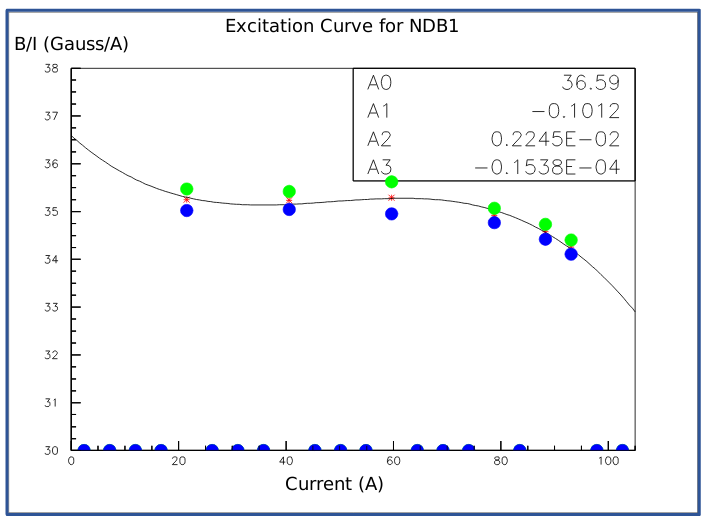
\includegraphics[height=3.0in]{figures/ExcitationCurves.png}
\caption{
{\scriptsize \sf Excitation Curve, B/I vs. I, for one NDB magnet, using two Hall probes (blue and green). Parameters from a cubic fit (black curve) to average of measurements (red) given in legend.}
}
\label{fig:magnet_excitation}
\end{centering}
\end{figure}

These magnets were air- and water-cooled during operations and their temperatures monitored. Due to concerns of overheating, the maximum usable field at the center of the magnets is $\sim$0.35 Tesla with 100 Amps of current being passed through the magnets.

%%%%%%%%%%%%%%%%%%%%%%%%%%%%%%%%%%%%%%%%%%%%%%%%%%%%%%%%%%%%
\subsubsection{Multi-Wire Proportional Chambers}\label{sec:MWPC}
%%%%%%%%%%%%%%%%%%%%%%%%%%%%%%%%%%%%%%%%%%%%%%%%%%%%%%%%%%%%
The wire chambers are based on the Fenker Chambers~\cite{Fenker} long in use at Fermilab.  The chambers have been upgraded by adding additional grounding to improve the signal to noise in the electronic readout.  The chambers, shown in Figure~\ref{fig:wirechamber}, have an effective aperture of 128~mm in both horizontal and vertical distances.  The wires are spaced at 1~mm, with 128 wires in each view.  In a test beam, the chambers have typical efficiencies of 98\% to 99\%. The gas used is 85\% Argon + 15\% isobutane.  The wire chambers typically operate between 2400 and 2500 volts.

\begin{figure}[!h]
\begin{centering}
\vspace{-0.3cm}
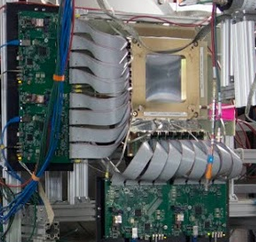
\includegraphics[height=2.3in]{figures/WireChamber.png}
\caption{
{\scriptsize \sf Image of one of the wire chambers used in the LArIAT tertiary beamline.}
}
\label{fig:wirechamber}
\end{centering}
\end{figure}

The front end amplifier/discriminator uses the ASDQ chip~\cite{ASDQchip}. Two of the ASDQ chips are mounted on a mother board that is plugged into the chamber.  Short flat cables are used to connect these ASDQ mother board to a new, multi-hit TDC~\cite{Sten}. This TDC provides a (maskable) fast OR output that can be used in a first level trigger. 

This TDC can accept multiple hits per wire with a time resolution of 1.18~ns/bin.  The TDCs can accept 2 edges per 9~ns.  The maximum event rate that can be accepted by the chamber system is of the order of one megahertz.  These limitations are clearly not an issue for the LArIAT beamline where the rates and timing resolution required are much less stringent than this.  There is enough memory on the TDC board to buffer a full spill of data (up to about 100 events/spill).  As in this application the spills occur only once per minute, there is ample time to read out the whole spill through a controller specially designed to support these TDCs.  Power and data flow to and from the controller to the TDCs and from the controller to the rest of the DAQ is via LVDS.  The time window for acceptance for hits, time offsets, front end threshold, and pulse shaping parameters may be programmed through the controller via a USB link from a PC or through an Ethernet connection.
 

%%%%%%%%%%%%%%%%%%%%%%%%%%%%%%%%%%%%%%%%%%%%%%%%%%%%%%%%%%%%
\subsubsection{Aerogel Cherenkov Detectors}\label{sec:Aerogel}
%%%%%%%%%%%%%%%%%%%%%%%%%%%%%%%%%%%%%%%%%%%%%%%%%%%%%%%%%%%%

Aerogel is an ultra-light material in which the liquid component of the gel has been replaced with a gas. The result is a solid with extremely low density, low thermal conductivity, and low index of refraction. The goal of having an aerogel threshold Cherenkov detector in the LArIAT beam line is to separate muons and pions in the momentum range where muons emit Cherenkov radiation while pions do not. This technique was demonstrated by the MICE and Belle II experiments ~\cite{MICE-aerogel,BelleII-aerogel} and in LArIAT we use two aerogel threshold Cherenkov detector with index of refraction of 1.057 and 1.103. Having different indices of aerogel allows LArIAT to do this separation in two different momentum ranges of interest.

\begin{figure}[htb]
\centering
\includegraphics[height=1.85in]{figures/Aerogel1103Figure.png}
\hspace{1cm}
\includegraphics[height=1.85in]{figures/Aerogel1057Figure.png}
\caption{Number of photoelectrons per cm versus momentum for the two indices of refraction that are employed by the LArIAT aerogel detectors. The photoelectron yield includes the response of a bialkali photocathode following the recipe in ~\cite{bib8}. }
\end{figure}


%%% KEK couter
The Aerogel Threshold Cherenkov Detector with the refractive index of 1.103 is placed just behind the second collimator on the tertiary beam line, between the two downstream wire chambers.
Figure~\ref{fig:kek_aerogel} is a picture of this aerogel detector.
It consists of 7 aerogel tiles (totaling 110 mm long in the beam direction), and the cross section of the detector is 108 mm $\times$ 108 mm.
The array of the aerogel tiles is wrapped with a diffusion sheet and viewed by two PMTs (HAMAMATSU R329-02) from the sides.
Figure~\ref{fig:kek_aerogel_ly} shows the observed light yield distribution for 550-800~MeV pions hitting the middle of the detector.
The obtained light yield is equivalent to 22 photoelectrons for $\beta=1$.
The fake rate for particles with velocity below the Cherenkov threshold is measured to be around 0.5\% with the threshold of 1.5 photoelectrons.

\begin{figure}[htb]
\centering
\includegraphics[height=1.85in]{figures/kek_aerogel.jpg}
\caption{The Aerogel Threshold Cherenkov Detector with the refractive index of 1.103.}
\label{fig:kek_aerogel}
\end{figure}

\begin{figure}[h]
\centering
\includegraphics[height=1.85in]{figures/kek_aerogel_ly.png}
\caption{The observed light yield distribution for 550-800 MeV pions hitting the middle of the detector.
The obtained light yield is equivalent to 22 photoelectrons for $\beta=1$.}
\label{fig:kek_aerogel_ly}
\end{figure}

%%%%%%%%%%%%%%%%%%%%%%%%%%%%%%%%%%%%%%%%%%%%%%%%%%%%%%%%%%%%
\subsubsection{Punch-Through and Muon Range Stack Instruments}\label{sec:MuRS}
%%%%%%%%%%%%%%%%%%%%%%%%%%%%%%%%%%%%%%%%%%%%%%%%%%%%%%%%%%%%
\input{muon-Punch.tex}


%%%%%%%%%%%%%%%%%%%%%%%%%%%%%%%%%%%%%%%%%%%%%%%%%%%%%%%%%%%%
\subsection{LArIAT Cosmic Ray Paddle Detectors}\label{sec:CosmicRayPaddle}
%%%%%%%%%%%%%%%%%%%%%%%%%%%%%%%%%%%%%%%%%%%%%%%%%%%%%%%%%%%%

LArIAT's system to trigger on cosmic rays is based on two so-called "cosmic towers" which stand  upstream and downstream of the cryostat, one on beam's right and one on beam's left, framing the cryostat.  Each cosmic tower is composed of two paddle assemblies, upper and lower.  The paddle assemblies each consist of four paddles, a matched pair which stand upright and a second matched pair lying across the top  of the assembly, to act as a veto for downward-going cosmic ray air showers.  Unless vetoes by the horizontal paddles, signals from paddle assemblies along the body diagonals of the TPC are combined in a logical ``AND'' to select cosmic muons crossing the TPC along one of its diagonals. A high proportion of events triggered this way contain cosmic ray tracks crossing both anode and cathode.  Such tracks provide a sample of LAr ionization with effectively uniform linear ionization density, but experience the entire range of charge attenuation available in the TPC before they drift to the anode. These tracks are used to calculate and monitor the level of electronegative contaminants in the liquid argon and provide a calibration sample for calorimetry and electric field studies outlined in Section \ref{sec:DetectorPerformance}.

The paddles have trapezoidal shape and are each enclosed in an aluminum case. An example is shown in Fig. \ref{pic:cosmicpaddle}. They come in two different sizes: a smaller version, with bases $32.2~cm$ and $26.7~cm$, $61.0~cm$ height and $3.02~cm$ thickness, and a bigger version, with bases $33.2~cm$ and $27.0~cm$, $70.8~cm$ height and $3.02~cm$ thickness. Each paddle is equipped with wavelength-shifting optical fibers running along one of the long sides and optically coupled to a low voltage, Zener-diode Hamamatsu H5783 PMT.  Signals from the PMT are amplified and discriminated by a custom-made PMT Amplifier and Discrimination (PAD) circuit mounted at one end of the paddle, then sent through a CAT5 cable to a Control and Concentrator Unit (CCU) which both power the PMT, controlling voltage and threshold, and output the PMT signal as logic ECL pulse.

\begin{figure}[h!]
 \centering
 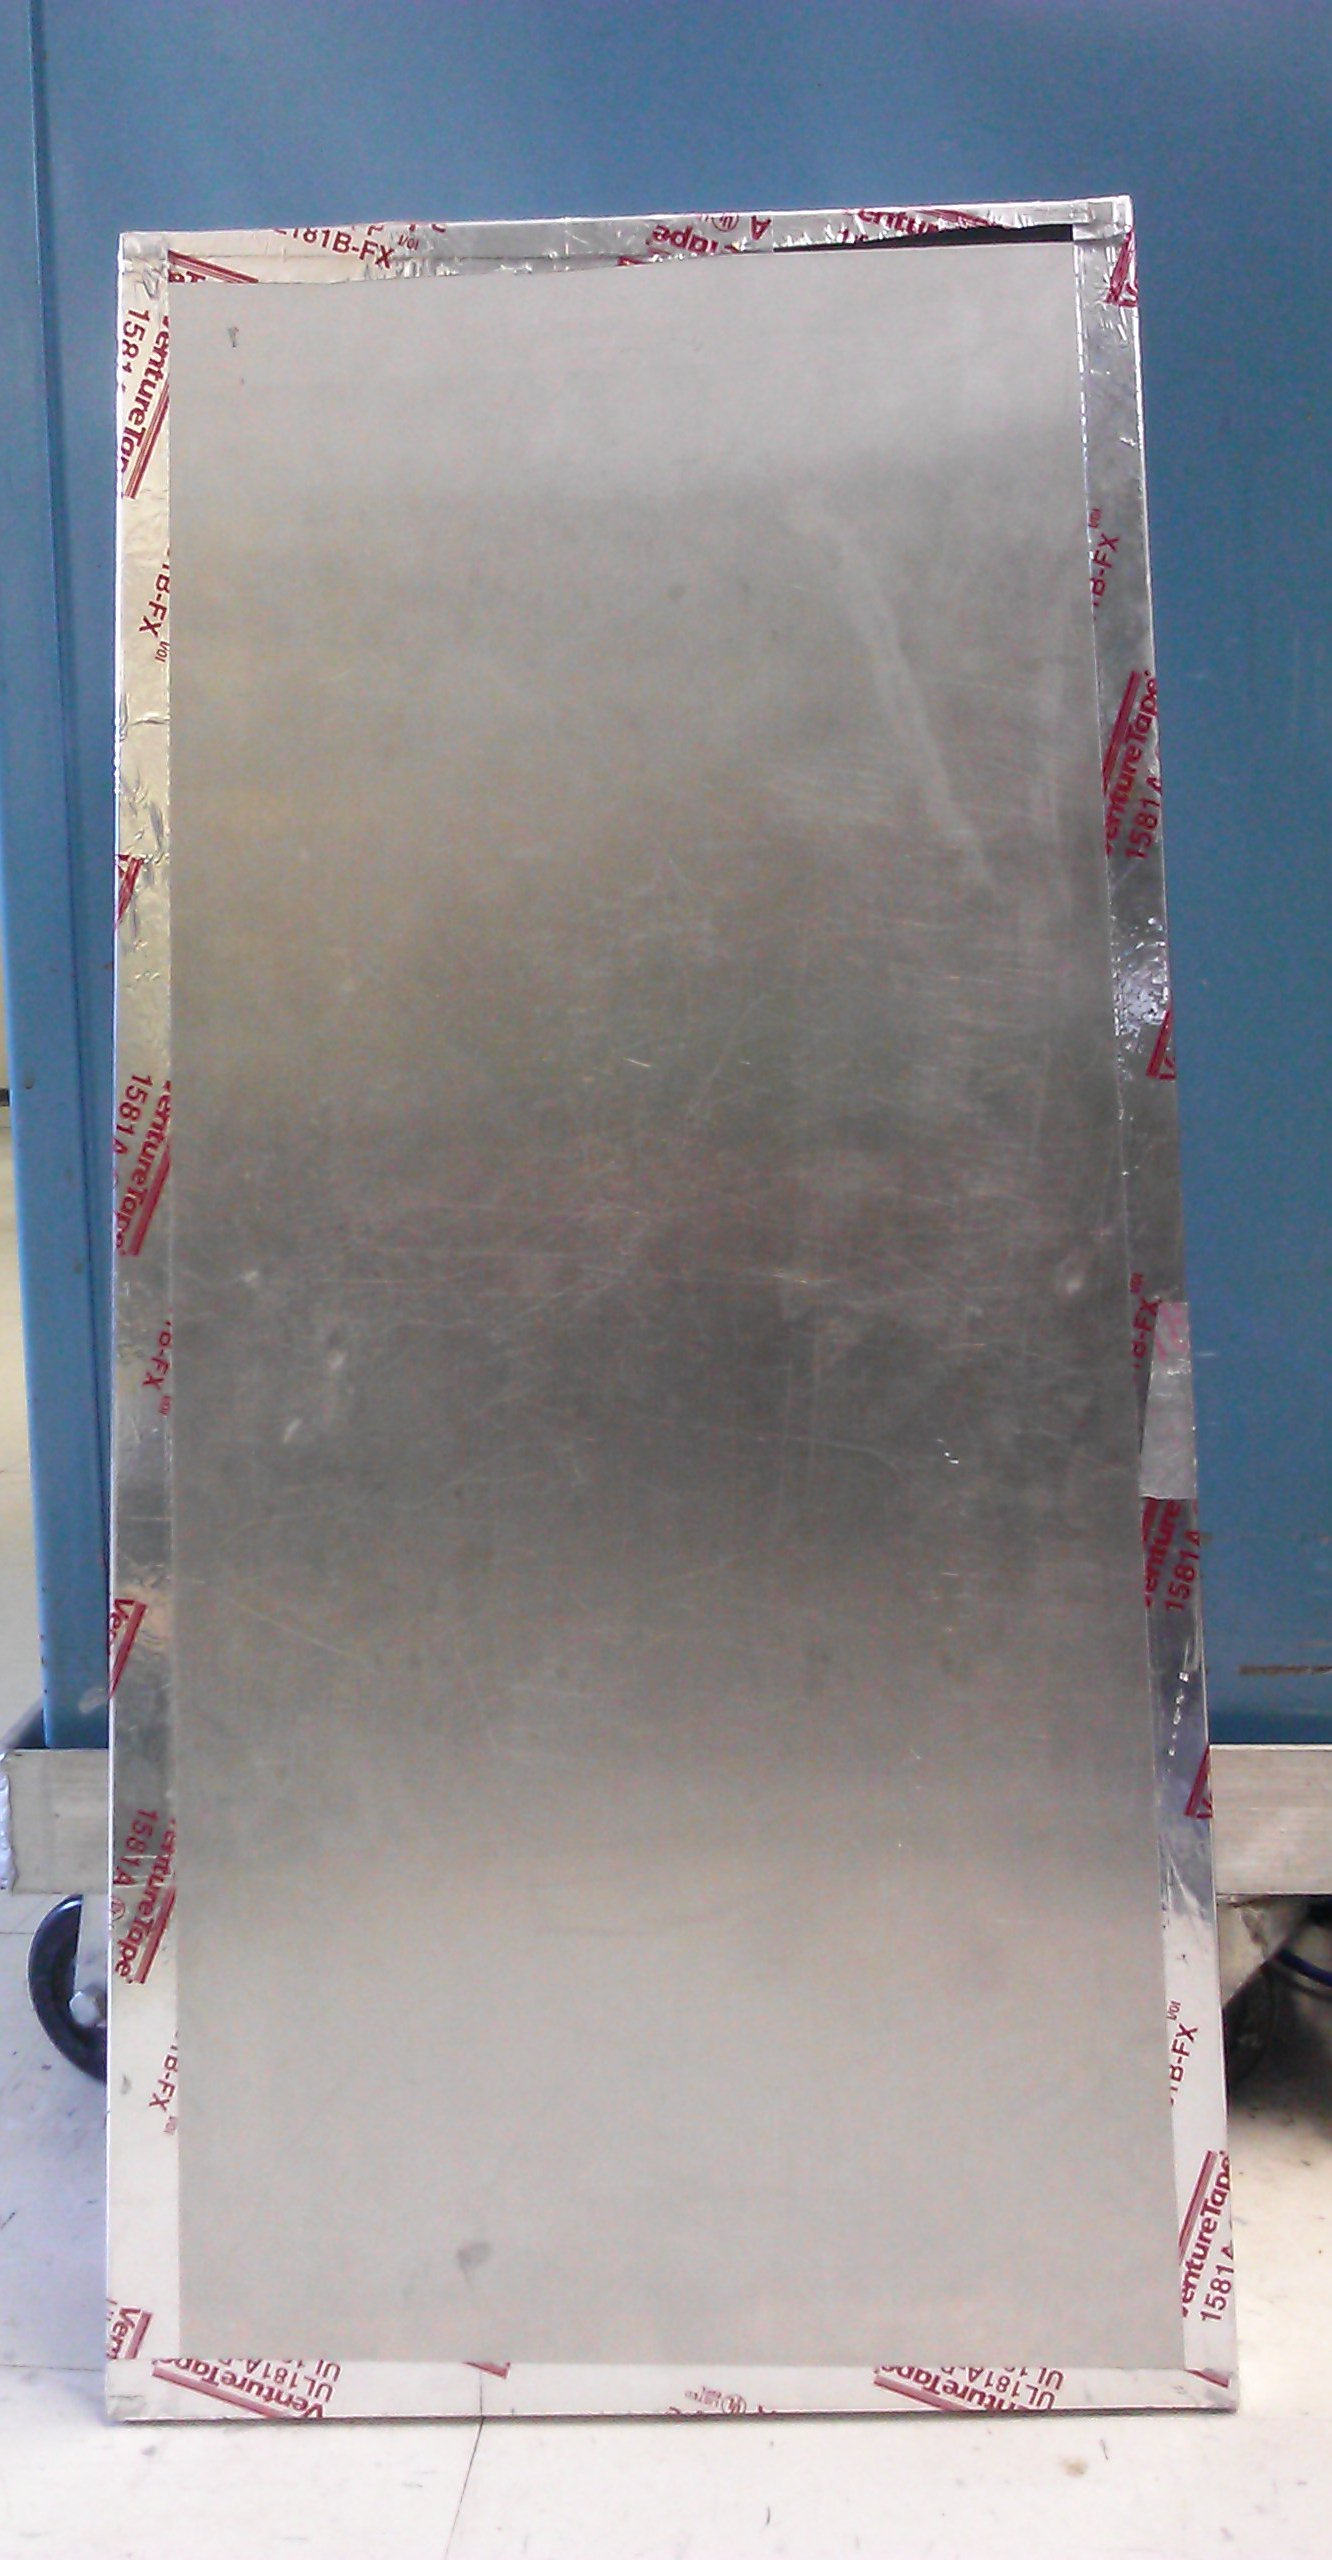
\includegraphics[angle=90,width=0.7\textwidth]{figures/Cosmic_Paddle.jpg}
\caption{
Photograph of one of the scintillation counters used in the cosmic towers. 
} 
\label{pic:cosmicpaddle}
\end{figure}

The paddles were selected from a pool of over 300 scintillating counters collected during the decommissioning of the CDF detector at Fermilab. 
For each counter, both the efficiency $\varepsilon_P$ and the noise $\eta_P$ as a function of the voltage were determined. The measurement was performed sandwiching the given paddle among 4 sample counters, placed two above and two below the paddle under test. The efficiency 
$\varepsilon_P$ was defined as the ratio between the 5-fold coincidence and the 4-fold coincidence of the sample counters. The accidental rate $\eta_P$ was instead defined as the number of 5-fold coincidence observed during ten minutes of data acquisition, when the signal of the paddle under test was delayed by $5 \mu s$. Each paddle with $\varepsilon_P \geq 95\%$ and $\eta_P = 0$ at working voltage was identified as a candidate for the Cosmic Ray system. The ones with the highest efficiency and lowest single count rate were then selected to realize the system itself. 
The plot of $\varepsilon_P$ as a function of the PMT voltage for one example paddle is shown in Fig. \ref{pic:CR_Effplot}.

\begin{figure}[h!]
 \centering
 \includegraphics[width=0.7\textwidth]{figures/TSU29_Efficiency.png}
\caption{
Plot of the counter efficiency $\varepsilon_P$ as a function of the PMT voltage for one of the paddles composing the Cosmic Ray system. 
} 
\label{pic:CR_Effplot}
\end{figure}


%$\varepsilon_P$ at a given voltage is defined as:

%$$
%\varepsilon_P = \frac{R_{1-2} \land R_{3-4} \land R_P}{R_{1-2} \land R_{3-4}}
%$$

%where $R_P$ is the rate of the paddle $P$ to be tested, $R_{1-2}$ is the coincidence rate of two sample paddles positioned above $P$, while $R_{3-4}$ is the coincidence rate of two sample paddles positioned below $P$.
%$\eta_P$ at a given voltage is instead defined as:

%$$
%\eta_P = \frac{R_{1-2} \land R_{3-4} \land R_{P^*}}{R_{1-2} \land R_{3-4}}
%$$

%where $R_{P^*}$ is the Rate of the paddle $P$ 


The trigger rate $R$ of the whole system is $R=0.032Hz$, corresponding to $\sim 1.9~\mu/minute$.



\section{The LArIAT Detector}\label{sec:LArIATDetector}

An Intro paragraph, as Will F. suggested, would be good here at the start of section 3. I might also rename this section to ?The LArIAT LArTPC Detector?, since beam line stuff is also ?The LArIAT Detector?.


%%%%%%%%%%%%%%%%%%%%%%%%%%%%%%%%%%%%%%%%%%%%%%%%%%%%%%%%%%%%
\subsection{Cryogenics}\label{sec:Cryo}
%%%%%%%%%%%%%%%%%%%%%%%%%%%%%%%%%%%%%%%%%%%%%%%%%%%%%%%%%%%%
\input{CryoDetails.tex}

%%%%%%%%%%%%%%%%%%%%%%%%%%%%%%%%%%%%%%%%%%%%%%%%%%%%%%%%%%%%
\subsection{Time Projection Chamber}\label{sec:TPC}
%%%%%%%%%%%%%%%%%%%%%%%%%%%%%%%%%%%%%%%%%%%%%%%%%%%%%%%%%%%%
\input{TPCDetails.tex}

%%%%%%%%%%%%%%%%%%%%%%%%%%%%%%%%%%%%%%%%%%%%%%%%%%%%%%%%%%%%
\subsection{TPC Electronics}\label{sec:MSUElectronics}
%%%%%%%%%%%%%%%%%%%%%%%%%%%%%%%%%%%%%%%%%%%%%%%%%%%%%%%%%%%%
\input{TPCelectronics.tex}

%%%%%%%%%%%%%%%%%%%%%%%%%%%%%%%%%%%%%%%%%%%%%%%%%%%%%%%%%%%%
\subsection{Digitization}\label{sec:Digitization}
%%%%%%%%%%%%%%%%%%%%%%%%%%%%%%%%%%%%%%%%%%%%%%%%%%%%%%%%%%%%
\input{Digitization.tex}

%%%%%%%%%%%%%%%%%%%%%%%%%%%%%%%%%%%%%%%%%%%%%%%%%%%%%%%%%%%%
\subsection{Trigger and Readout System}\label{sec:Trigger}
%%%%%%%%%%%%%%%%%%%%%%%%%%%%%%%%%%%%%%%%%%%%%%%%%%%%%%%%%%%%
\input{Trigger.tex}

%%%%%%%%%%%%%%%%%%%%%%%%%%%%%%%%%%%%%%%%%%%%%%%%%%%%%%%%%%%%
\subsection{Photon Detection System}\label{sec:PhotonSystem}
%%%%%%%%%%%%%%%%%%%%%%%%%%%%%%%%%%%%%%%%%%%%%%%%%%%%%%%%%%%%
\input{LightDetectionSystem.tex}


The LArIAT cryogenic system consists of the repurposed ArgoNeuT cryostat, the new process piping, and a liquid argon filtration system installed at Fermilab's Test Beam Facility.

%%%%%%%%%%%%%%%%%%%%%%%%%%%%%%%%%%%%%%%%%%%%
\begin{subsubsection}{Cryostat}
%%%%%%%%%%%%%%%%%%%%%%%%%%%%%%%%%%%%%%%%%%%%
The LArIAT cryostat, shown in Figure \ref{fig:LArIATCryoStat}, was repurposed from the ArgoNeuT experiment with a series of modifications to allow for operations in a charged particle test beam. The cryostat \cite{ArgoNeuT} consists of an inner volume containing the purified liquid argon and an outer volume serving as a vacuum jacket with layers of aluminized mylar superinsulation. Both the inner and outer cryostat vessels are cylindrical in shape with convex end caps.  Access to the internal volume is possible by opening the upstream end caps of the inner and outer vessels. The main axis of the cryostat is horizontal and oriented parallel to the beam. The inner vessel is 76.2~cm in diameter and 130~cm in length, corresponding to a liquid argon volume of about 550~L, or a mass of 0.76 t. The cryostat has a wide neck, or ``chimney'', protruding from its top at mid-length which serves as an access path for signal cables from the LArTPC and the internal instrumentation, as well as for the high voltage feedthrough. 

\begin{figure}[htb]
\centering
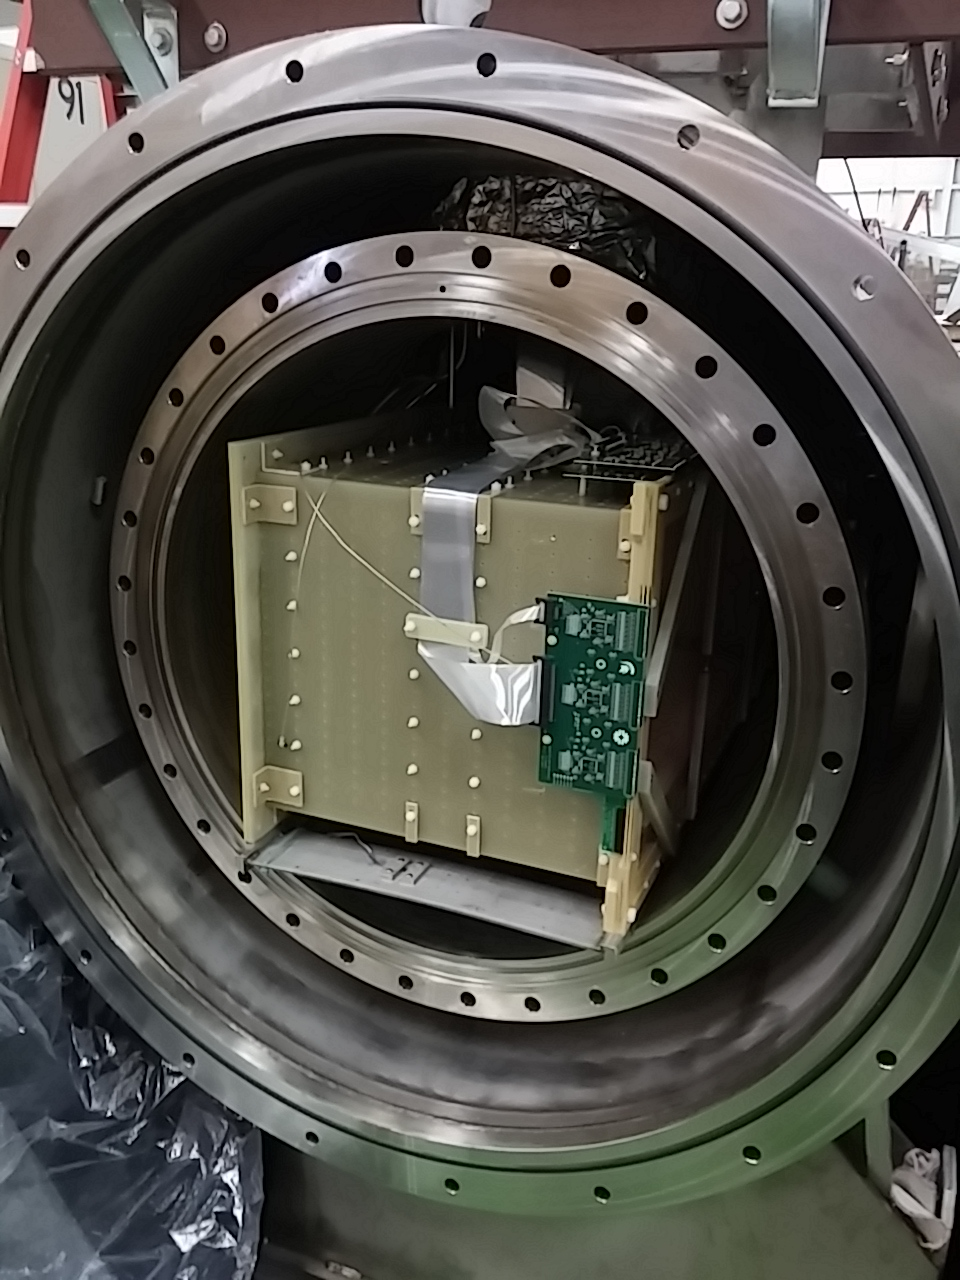
\includegraphics[scale=0.18]{./figures/Cryostat1.jpg}
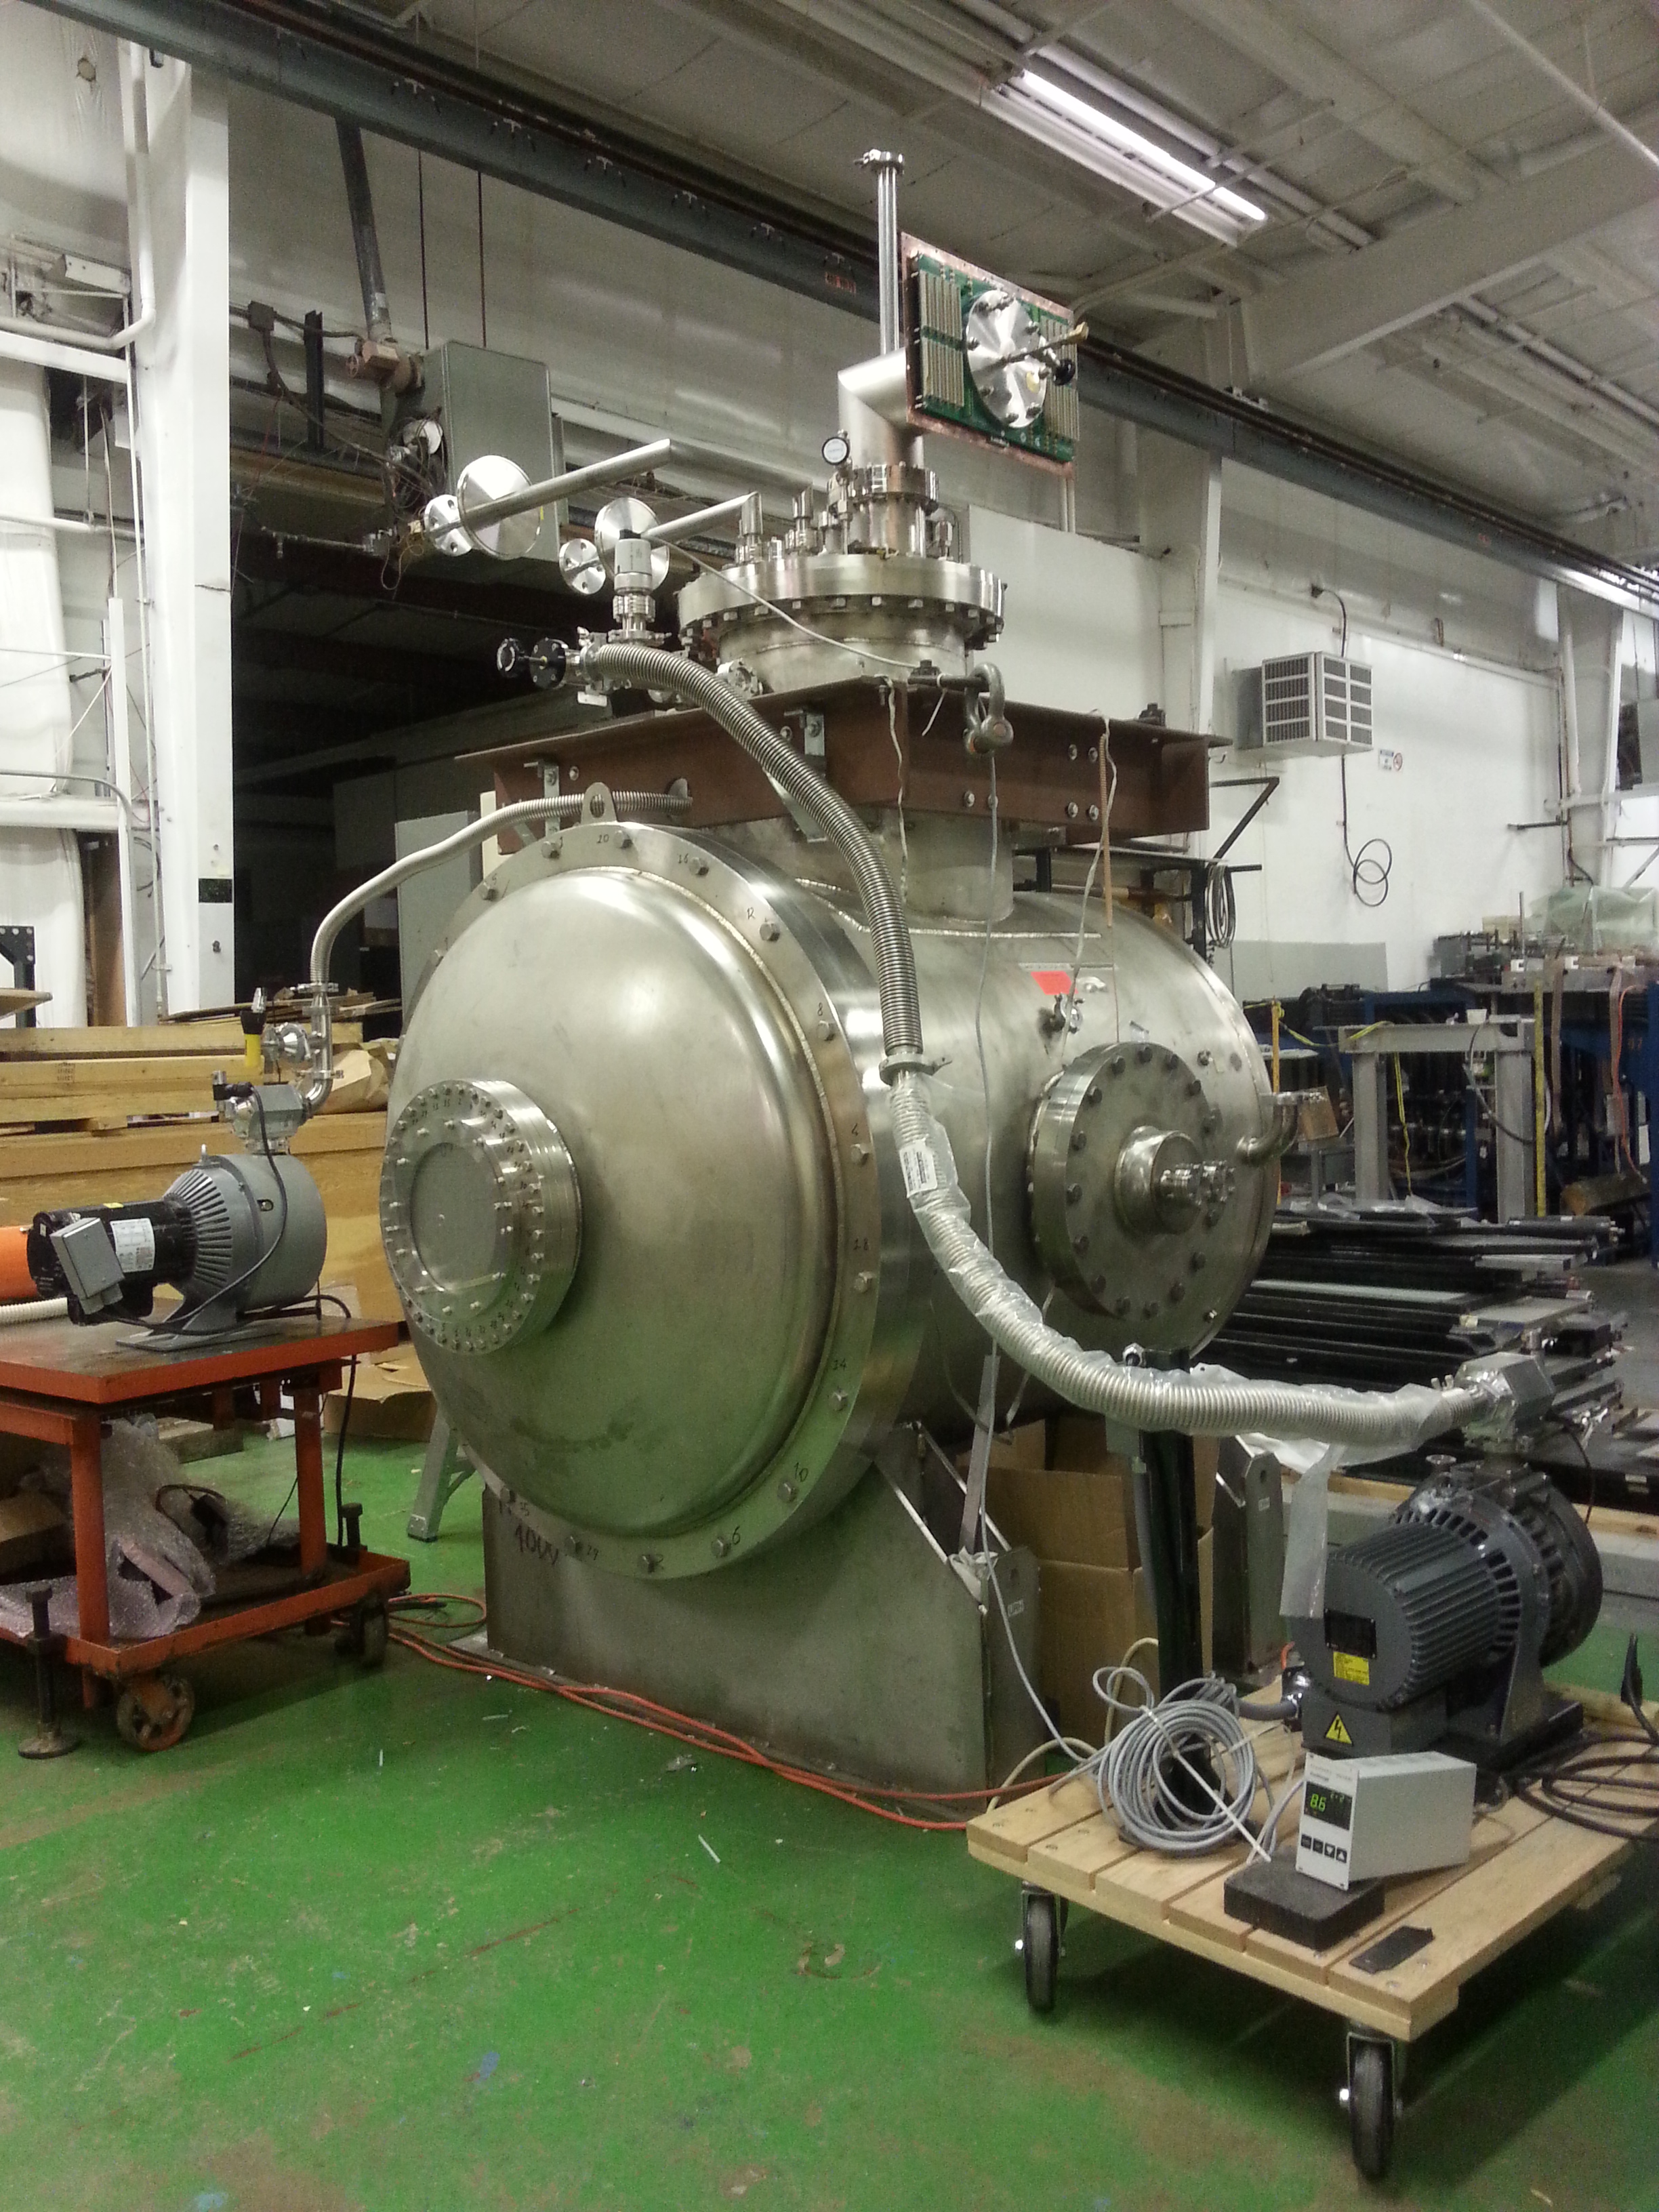
\includegraphics[scale=0.07]{./figures/Cryostat2.jpg}
\caption{\emph{(left)} The LArIAT cryostat open with the TPC placed in the inner volume. \emph{(right)} The LArIAT cryostat fully sealed during initial commissioning prior to installation at Fermilab Testbeam Facility.}
\label{fig:LArIATCryoStat}
\end{figure}

Several modifications to the cryostat were made to meet the requirements of operating in a charged particle test beam and to facilitate the new liquid argon purification system. These modifications, shown in Figure \ref{fig:LArIATCryoMods}, include:
\begin{enumerate}[label=\roman*),topsep=0pt,itemsep=-1ex,partopsep=1ex,parsep=1ex]
\item A ``beam window'' on the front outer end cap and an ``excluder'' on the inner endcap.  The purpose of these modifications is to minimize the amount of material upstream of the TPC's active volume along the beam line.  On the original ArgoNeuT cryostat the stainless steel end caps of the cryostat's inner and outer vessels were 3/16'' (4.8 mm) thick. In addition, upstream of the TPC active volume there was a region of uninstrumented liquid argon approximately 15~cm in length. This corresponded to $\sim$ 1.6 radiation lengths ($X_{0}$) of dead material between the outside of the cryostat and the TPC, which would have impeded charged test beam particles prior to their entrance into the active volume.  To mitigate this effect, the 9'' (22.9~cm) diameter beam window located at the center of the outer vessel's front flange was installed along with a blanked 0.4~mm titanium sheet. On the inner vessel's end cap, a hollow concave volume (the ``excluder'') was installed to reduce the amount of liquid argon charged particles would traverse before reaching the active volume of the TPC. With these modificaitons in place, the total material thickness seen by charged particles entering the front face of the LArIAT cryostat is now less than 0.3 $X_{0}$. 
\item A connection for a liquid argon transfer line to the new argon cooling and purification system. This modification consists of an outlet at the bottom of the cryostat with Conflat and ISO flange sealing. 
\item The addition of side port feedthroughs to accomodate signal and high-voltage bias connections for the scintillation light detection system (described in more detail in Section \ref{sec:PhotonSystem}). Both the inner and outer cryostat vessels had their existing side ports modified with CF-flanged apertures to accomplish this.
\end{enumerate}

%$i)$ A ``beam window'' on the front outer end cap and an ``excluder'' on the inner endcap to minimize the amount of material upstream of the TPC's active volume along the beam line; $ii)$ a connection at the base of the cryostat for the argon cooling and purification system; and $iii)$ the addition of a side port feedthrough to accomodate bias and signal connections for the scintillation light detectors.


%On the original ArgoNeuT cryostat the stainless steel end caps of the cryostat's inner and outer vessels were 3/16'' (4.8 mm) thick. In addition, upstream of the TPC active volume there was a region of uninstrumented liquid argon approximately 15~cm in length. This corresponded to $\sim$ 1.6 radiation lengths ($X_{0}$) of dead material between the outside of the cryostat and the TPC, which would have impeded charged test beam particles prior to their entrance into the active volume.  To minimize the effect of this dead region, a 9'' (22.9~cm) diameter beam window located at the center of the outer vessel's front flange was installed along with a blanked 0.4~mm titanium sheet. On the inner vessel's end cap, a hollow concave volume (the ``excluder'') was installed to reduce the amount of liquid argon charged particles would traverse before reaching the active volume of the TPC. With these modificaitons in place, the total material thickness seen by charged particles entering the front face of the LArIAT cryostat is now less than 0.3 $X_{0}$. 

%The cryostat vessels were modified to connect a liquid argon transfer line to the new cooling and purification system. This modification consists of an outlet at the bottom of the cryostat with Conflat and ISO flange sealing. 

%Finally, both the inner and outer cryostat vessels had their existing side ports modified with CF-flanged apertures for the signal and high-voltage bias feedthroughs for the scintillation light system, described in more detail in Section \ref{sec:PhotonSystem}.

\begin{figure}[htb]
\centering
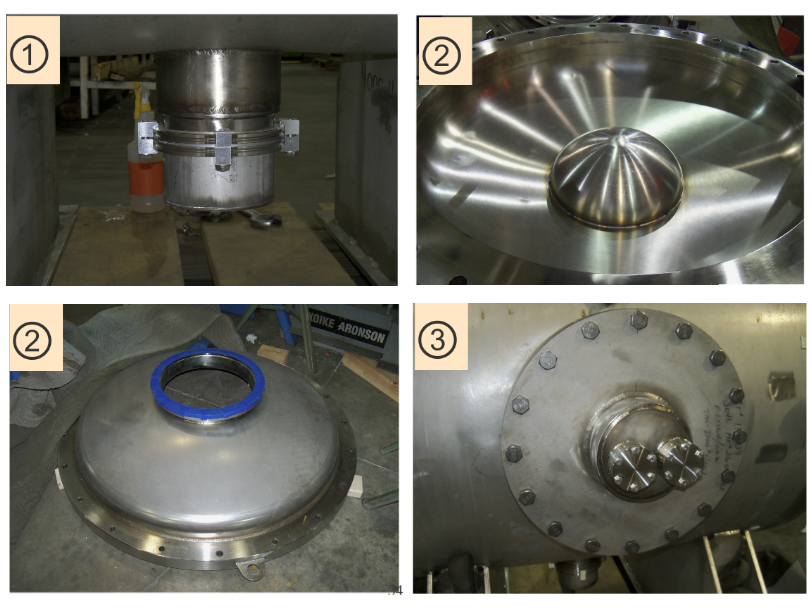
\includegraphics[scale=0.35]{./figures/CryoMods.png}
\caption{Pictures of the modified components of the cryostat. $1)$ The addition of an outlet to the bottom of the cryostat to allow connections to the purification system; $2)$ The ``beam-window'' on the outer endcap and the concave inner surface of the inner endcap (referred to as the excluder) to reduce the amount of material through which beam particles must travel before entering the TPC; $3)$ The modified side port for the LArIAT light collection system.}
\label{fig:LArIATCryoMods}
\end{figure}

\end{subsubsection}

%%%%%%%%%%%%%%%%%%%%%%%%%%%%%%%%%%%%%%%%%%%%
\begin{subsubsection}{Liquid Argon System}\label{sec:LArCryoSystem}
%%%%%%%%%%%%%%%%%%%%%%%%%%%%%%%%%%%%%%%%%%%%
LArIAT is supplied with liquid argon from a commercial dewar positioned outside of the experimental enclosure.  Liquid argon is delivered by a vendor with a specified maximum contamination of 2 parts per million (ppm) oxygen, 3.5~ppm water, and 10~ppm nitrogen. Oxygen and water contamination is detrimental to the ability of the ionization electrons to drift through the volume, as free electrons readily attach to these molecules. Nitrogen contamination is detrimental to the collection of scintillation light.  The level of these contaminants in the delivered argon is determined using a suite of commercial gas analyzers.  In practice, the delivered argon has much less than 1~ppm of all these contaminants.  Even such apparently low levels of contamination are too large to effectively drift ionization electrons, so filtration of the argon is required to achieve oxygen and water contamination at the level of 100 parts per trillion (ppt) or better. %{\bf 100 ppt is sufficient for a 3 ms lifetime, I think LArIAT has less than that}.

The argon is delivered from the commercial dewar to the cryostat through 2.54~cm diameter schedule 10 stainless steel piping.  The piping was insulated with 20.32~cm of polyurethane foam by the manufacturer.  The piping was cleaned to remove oil and grease before being welded into the system. The argon then passes through LArIAT's argon filtration system which is based on the Liquid Argon Purity Demonstrator (LAPD)~\cite{LAPD} design. The purification system consists of a single 77~liter filter which is filled halfway with a 4A molecular sieve supplied by Sigma-Aldrich~\cite{sigma-aldrich} that primarily removes water contamination but can also remove small amounts of nitrogen and oxygen. The remaining volume of the filter contains BASF~CU-0226~S, a highly dispersed copper oxide impregnated on a high surface area alumina, to remove oxygen~\cite{basf} and to a lesser extent, water.  The filter is insulated with a vacuum jacket and aluminum radiation shields.  The filter media are regenerated in place using heated gas, as was done for LAPD. The filter media are very efficient at removing oxygen and water and the argon is pure enough after a single pass through the media to allow several millisecond electron drift lifetimes in the TPC. 

From the filter the argon is directed into the inner cryostat via a liquid feedthrough on the top of the cryostat. The argon level, temperatures, and pressures are continuously monitored during operation both in the commercial dewar supplying the argon as well as the levels inside the cryostat, as shown on the top of Figure \ref{fig:LArIATCryoMonitor}. The argon in the cryostat is allowed to boil and vent to the atmosphere during operation and the argon level is monitored via the level probes. Flow of argon into the cryostat is enabled whenever the liquid level goes below a predetermined value to ensure that the TPC high voltage feedthrough and cold electronics are always submerged. During normal operations, the liquid level inside the cryostat is replenished several times per day, as can be seen by the cycle of the liquid level and valve positions shown at the bottom of Figure \ref{fig:LArIATCryoMonitor} 

\begin{figure}[htb]
\centering
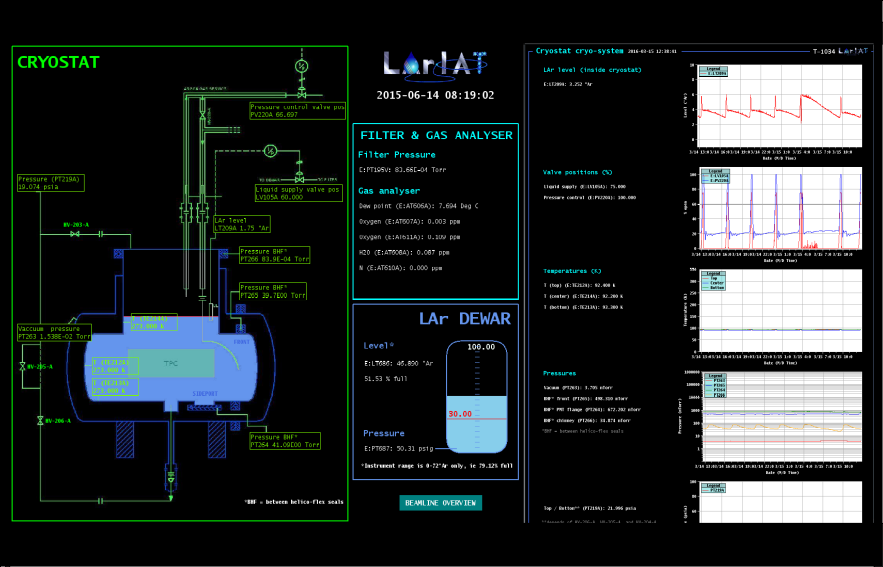
\includegraphics[scale=0.35]{./figures/CryoMonitor.png}
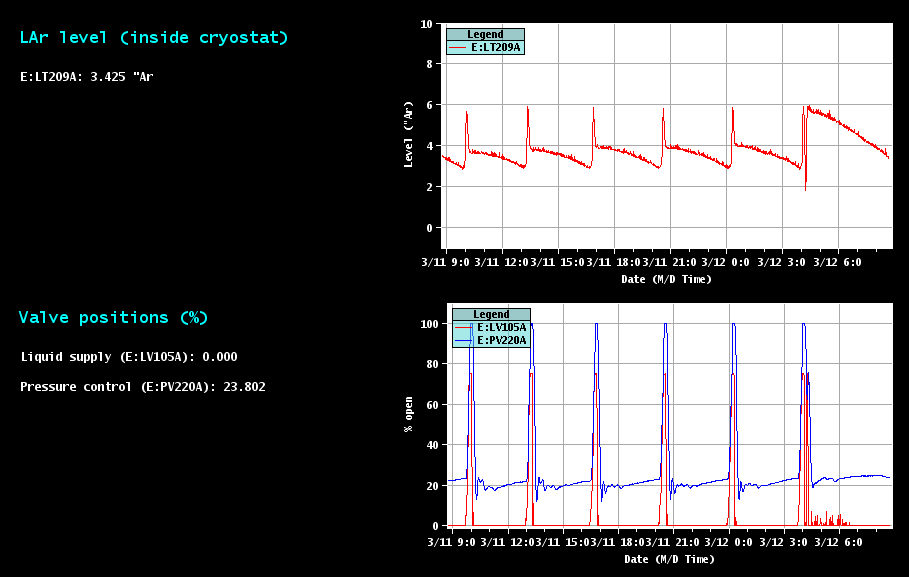
\includegraphics[scale=0.34]{./figures/CryoMonitor2.png}
\caption{\emph{(top)} Screenshot of the LArIAT cyrosystem monitoring page showing the levels of the argon both inside the cryostat and in the supply dewar as well as the monitored levels plotted over a twenty-four hour period. \emph{(bottom)} Plots showing the liquid argon level inside the cryostat as well as the corresponding liquid valve which allows argon to flow into the cryostat and the level drops due to boiling. The frequency of the typical fill/vent cycle can be seen with the typical time between fills being slightly more than 3 hours.}
\label{fig:LArIATCryoMonitor}
\end{figure}


The temperature of the argon inside the cryostat can be determined through direct use of temperature probes deployed at the bottom, middle, and top of the cryostat (listed as TE213A, TE314A, and TE212A in Figure \ref{fig:LArIATCryoMonitor} respectively). This can be crossed check using the pressure in the cryostat gas volume and extrapoloting this to the center of the liquid volume. The pressure at the surface of the liquid argon is maintained by the cryosystem at $\sim$20~psi $\pm$.0.4 psi.

In order to determine the temperature inside the TPC, we measure the pressure in the cryostat gas volume and calculate the pressure at the center of the TPC. From this pressure and the boiling point curve of argon, we calculate the temperature. The pressure at the surface of the liquid argon is maintained by the cryosystem at $\sim$20~psi as shown in Figure \ref{fig:pressure} for a period of 13 days with an average pressure of 20.0 $\pm$.0.4 psi. If we consider approximately 40 cm of argon from the ulage surface to the center of the TPC this would give the pressure there of $\sim$20.8 psi, which according to the Reference \cite{} corresponds to a temperature of 90.7 K. This is consistent with the readings given of the temperature probes, shown in Table \ref{tab:temp}. This cross-check both provides a basis for the electron mobility calculation used when calibrating the drift speed, as is discussed in Section \ref{}, as well as providing confidence in the monitoring tools.


\begin{table}[h!]
\centering
\caption{Average temperatures measured at the top, middle and bottom in the LArIAT cryostat.}
\label{tab:temp}
\begin{tabular}{|c|c|c|}
\hline
Top Probe Temp (TE212A) & Middle Probe Temp (TE214A)   & Bottom Probe Temp (TE213A)  \\ \hline
91.7 $\pm$ 0.7 K &  91.8 $\pm$ 0.7 K                   & 93.3 $\pm$ 2.7 K       \\ \hline
\end{tabular}
\end{table}


\end{subsubsection}
The Liquid Argon Time Projection Chamber (LArTPC) can be broken down into three major subcomponents: $1)$ The high voltage system which provides the drift field voltage; $2)$ the cathode and field cage which steps down the high voltage through a network of voltage-dividing resistors to form a uniform electric field for charges to drift within; and $3)$ the wire planes which provide the charge sensitive readout for the detector. Here we describe each of the subcomponents which make up the LArIAT LArTPC.

%%%%%%%%%%%%%%%%%%%%%%%%%%%%%%%%%%%%%%%%%%%%
\begin{subsubsection}{High Voltage}\label{sec:DriftVoltage}
%%%%%%%%%%%%%%%%%%%%%%%%%%%%%%%%%%%%%%%%%%%%
The drift high voltage system for the LArIAT detector, shown pictorially in Figure~\ref{fig:HVScheme}, is designed to allow ionization electrons from the interaction of charged particles in the liquid argon to drift to the wireplanes. The high voltage system consists of a Glassman LX125N16 power supply~\cite{GlassmanPS} capable of generating -125~kV and 16~mA of current. This power supply was typically operated much below this limit during normal data taking operations. The voltage from the power supply is transmitted through high voltage cables to a series of filter pots before finally reaching the high-voltage feedthrough on the top of the LArIAT cryostat. This feedthrough brings the voltage into the liquid argon volume to be transmitted to the TPC cathode.


\begin{figure}[htb]
\centering
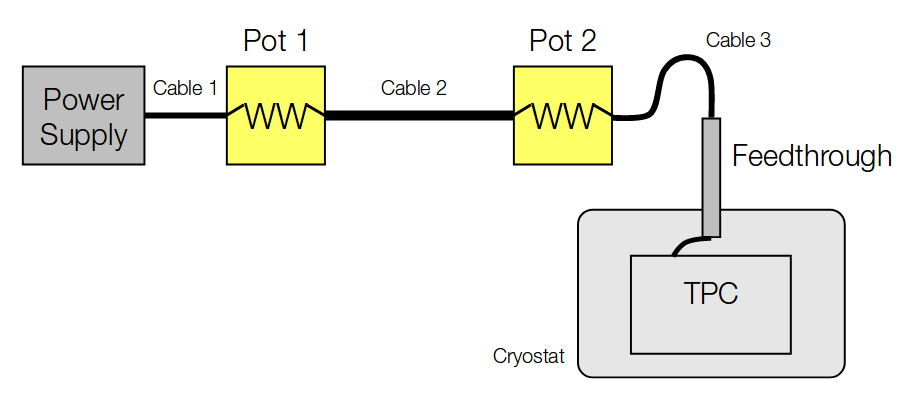
\includegraphics[scale=0.35]{./figures/HVSchematic.png}\\
\caption{Schematic of the LArIAT high voltage system.}
\label{fig:HVScheme}
\end{figure}%See DocDB 1472

The first high voltage cable which connects the Glassman power supply to the first filter pot is a 1/2-inch HV cable, Glassman cable model 2121, supplied by the Glassman manufacturer. The second cable is a $\sim$100-ft long 1/2-inch Type-2134 Dielectric Sciences cable which connects the first filter pot to the second filter pot. Finally, the same type of cable is used to connect the second filter pot to the high voltage feedthrough at the cryostat.

The two filter pots that are inline with the high voltage system serve to: $a)$ limit the current draw on the power supply; $b)$  provide a low-pass filter to help reduce the voltage ripple on the cathode; and $c)$ partition the energy stored in the system in the event of a high voltage trip. Each filter pot, as shown in Figure~\ref{fig:FilterPot}, is a cylindrical aluminum pot 18.5 inches tall by 20 inches in diameter and 3/16 inches thick, with welded tops each having an opening that allows for a flange and o-ring to receive the high voltage cables. Within each pot, the flanges are connected to four 10~M$\Omega$ resistors connected in series. This assembly is submerged in $\sim$16 gallons of Diala transformer oil~\cite{ShellDiala} to aid in the suppression of corona and discharges.

\begin{figure}[htb]
\centering
\includegraphics[scale=0.35]{./figures/FilterPot.png}\\
\caption{Filter pots used in the LArIAT high voltage system.}
\label{fig:FilterPot}
\end{figure}%See DocDB 1472

The final piece of the high voltage system is the high voltage feedthrough which delivers the drift voltage to the cathode of the TPC. This feedthrough is based on a a custom design that was used by ICARUS \cite{IcarusDetector}. The feedthrough consists of a stainless steel inner conductor surrounded by a tube of ultra high molecular weight polyethylene further surrounded by a stainless steel outer ground tube. The high-voltage feedthrough enters the cryostat from a dedicated 4-5/8 inch Conflat flange at the top of the cryostat. The end of the inner conductor is finally attached to the cathode by a flexible conductor bolted at both ends. A technical drawing of the LArIAt high voltage feedthrough can be found in Figure \ref{fig:HVFT}. 

\begin{figure}[htb]
\centering
\includegraphics[scale=0.35]{./figures/lariatFeedthrough.pdf}\\
\caption{Technical drawing of the LArIAT high voltage feedthrough. Various liquid argon levels are shown in cyan to indicate the levels to ensure the feedthrough is immersed in argon during operations}
\label{fig:HVFT}
\end{figure}%See DocDB 1472

During usual operations, the operating voltage from the Glassman power supply was -23.5~kV corresponding to a drift field of $\sim$500 V/cm. During special runs, the high voltage system was operated in a range from 0~kV to 32.8~kV (corresponding to drift fields ranging from 0~V/cm to 700~V/cm) and the feedthrough was tested up to 60~kV with no electrical breakdown observed.


\end{subsubsection}

%%%%%%%%%%%%%%%%%%%%%%%%%%%%%%%%%%%%%%%%%%%%
\begin{subsubsection}{Cathode and Field Cage}\label{sec:FieldCage}
%%%%%%%%%%%%%%%%%%%%%%%%%%%%%%%%%%%%%%%%%%%%

\textcolor{red}{Description of the cathode and field cage is missing}

As shown in Figure \ref{fig:driftregions}, the LArIAT TPC has three drift volumes, each of which has its own electric field. The main drift volume is defined as the region between the cathode plane and the shield plane (C-S). Note that the shield plane wires are \emph{not} read out. The other two drift regions are those between the shield plane and the induction plane (S-I), and between the induction plane and the collection plane (I-C). The electric field in these regions is chosen to satisfy the charge transparency condition to allow for 100$\%$ transmission of the drifting electrons through the shield and then the induction planes. We provide a detailed description of the electric field measurement in each region in \ref{sec:EFieldMeasurements}.

\begin{figure}[htb]
\centering
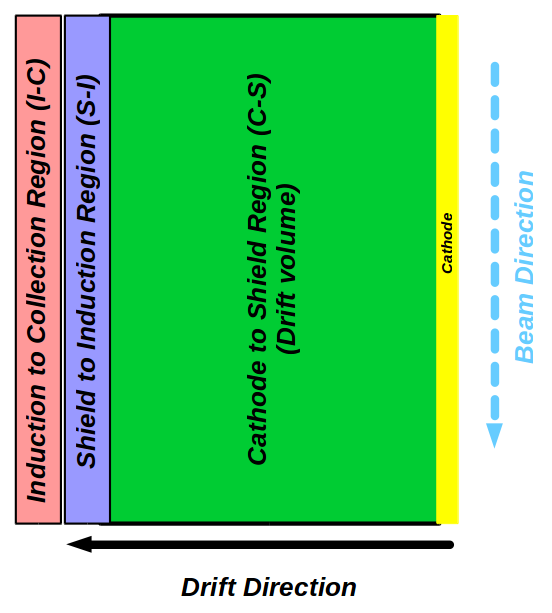
\includegraphics[scale=0.35]{./images/DriftRegions.png}\\
\caption{Schematic of the three drift regions inside the LArIAT TPC: the main drift volume between the cathode and the shield plane (C-S) in green, the region between the shield plane and the induction plane (S-I) in purple, and the region between the induction plane and the collection plane (I-C) in pink.}
\label{fig:driftregions}
\end{figure}

Table \ref{tab:voltages} provides the default voltages applied to the cathode and the shield, induction, and collection plane for all the runs. These voltages were tuned to maintain the transparency condition when the (I-C) and (S-I) spacing changed. For data taken in Run-I, Run-II, and Run-IIIb the spacing was a constant 4~mm; the spacing was 5~mm for Run-IIIa. 

\begin{table}[htpb]
\centering
\caption{Anode planes default voltages}
\label{tab:voltages}
\begin{tabular}{lllll}
\hline
\multicolumn{1}{|l|}{V Cathode} & 
\multicolumn{1}{|l|}{V Shield} & \multicolumn{1}{l|}{V Induction} & \multicolumn{1}{l|}{V Collection} & \multicolumn{1}{|l|}{Run} \\ \hline
\multicolumn{1}{|l|}{-23.17 kV} &
\multicolumn{1}{|l|}{-298.8 V} & \multicolumn{1}{l|}{-18.5 V}      & \multicolumn{1}{l|}{338.5 V} & \multicolumn{1}{|l|}{Run-I, Run-II \& Run-IIIb}      \\ \hline
\multicolumn{1}{|l|}{-23.17 kV} & 
\multicolumn{1}{|l|}{-325.8 V} & \multicolumn{1}{l|}{-0.6 V}      & \multicolumn{1}{l|}{421.9 V} & \multicolumn{1}{|l|}{Run-IIIa}      \\ \hline

                              &                                 &                                 
\end{tabular}
\end{table}

\end{subsubsection}

%%%%%%%%%%%%%%%%%%%%%%%%%%%%%%%%%%%%%%%%%%%%
\begin{subsubsection}{Wire Plane Assembly}\label{sec:WirePlanes}
%%%%%%%%%%%%%%%%%%%%%%%%%%%%%%%%%%%%%%%%%%%%

%%%%%%%%%%%%%%%%%%%%%%%%%%%%%%%%%%%%%%%%%%%%
\begin{subsubsection}*{Wire Winding}
%%%%%%%%%%%%%%%%%%%%%%%%%%%%%%%%%%%%%%%%%%%%

Wires for the LArIAT wire planes are wound to the correct spacing and tension on an independent winding machine before being transferred to the printed circuit boards on which they are installed in the TPC.

\begin{figure}[h!]
\centering
\includegraphics[height=2in]{figures/MamaBear.jpg}
\caption{The wire-winding apparatus in action. Both frames are attached and a single wire has been wound.}
% CAN PROBABLY FIND A BETTER PICTURE!
\label{pic:mamabear}
\end{figure}

Two rectangular steel frames are bolted back-to-back on an apparatus that rotates at a constant speed, shown in Figure \ref{pic:mamabear}. As the frames rotate, wire is drawn from a spool and wrapped around the two frames at constant tension (monitored by a tensiometer in the device paying out the spool). Once the requisite number of wires have been wound, the wires are epoxied onto the steel frames with five-minute epoxy and cut, giving two separate wire planes (one on each frame).
\end{subsubsection}

%%%%%%%%%%%%%%%%%%%%%%%%%%%%%%%%%%%%%%%%%%%%
\begin{subsubsection}*{Wire Transfer}
%%%%%%%%%%%%%%%%%%%%%%%%%%%%%%%%%%%%%%%%%%%%
Once the wire planes have been wound, they must be transferred from the winding frames onto the G10 wire-carrier boards that go into the LArIAT TPC. To achieve this, the frames are unbolted from the winding apparatus and laid over the board onto which the wires are to be transferred, which itself is bolted to a rigid aluminium frame to prevent it from flexing under tension. Careful manual alignment is performed, using guide holes drilled in the board for reference. This alignment is shown in Figure \ref{pic:wiretransfer}.

Once the wires are aligned to the solder pads on the board, they are glued to the board behind the solder pads with a temporary epoxy strip (using five-minute epoxy) to preserve the alignment. This is then followed by a permanent epoxy strip on the inside of the solder pads, using a slow-curing epoxy that is safe for cryogenic conditions. This epoxy is allowed to cure for 12 to 24 hours before the wires are cut behind the temporary strip and the winding frame can be removed.

\begin{figure}[h!]
\centering
\includegraphics[height=2in]{figures/WireTransfer.jpg}
\caption{One of the \textcolor{red}{This can be 4mm or 5 mm wire plane} 3~mm wire planes during transfer, with the wires not yet cut from the winding frame. A steel bar was used for this plane to ensure all wires made good contact with the board.}
\label{pic:wiretransfer}
\end{figure}

\end{subsubsection}

%%%%%%%%%%%%%%%%%%%%%%%%%%%%%%%%%%%%%%%%%%%%%%%%%%%%%%%%%%%%%%%%%
\begin{subsubsection}*{Soldering of Electrical Connections}
%%%%%%%%%%%%%%%%%%%%%%%%%%%%%%%%%%%%%%%%%%%%%%%%%%%%%%%%%%%%%%%%%

When the wire transfer is complete, the wires are soldered to their pads using [SOLDER DETAILS HERE], as are the resistor and capacitor components for the U and V planes \textcolor{red}{Which are the values of capacitances and resistances?}. Mylar sheeting is used to protect the active region of the wire planes from evaporating solder flux during this process. Once all wires have been soldered in place, the wires are broken off behind the solder pads and the temporary epoxy strip is removed. The entire board is cleaned with ethyl alcohol to remove any residue of solder flux before the finished wire planes ahead of installation in the TPC.
\end{subsubsection}

%%%%%%%%%%%%%%%%%%%%%%%%%%%%%%%%%%%%%%%%%%%%%%%%%%%%%%%%%%%%%%%%%
\begin{subsubsection}*{Wire Plane Testing}
%%%%%%%%%%%%%%%%%%%%%%%%%%%%%%%%%%%%%%%%%%%%%%%%%%%%%%%%%%%%%%%%%

\textbf{Electrical Testing}\\
\textcolor{red}{Both the test on the RC and on the wire tension are very bad described. According to me it is better to delete the section if a better description can not be provided.}
Every channel on each completed plane is probed with a multimeter and a signal generator to check for electrical continuity, and in the case of the U and V planes, for the correct RC time constant from the components.\\
\textbf{Tension Testing}\\
A laser tensiometer is mounted on a rigid aluminium arm over each completed frame and used to verify the tension on a representative sample of the wires. [QUANTITATIVE RESULTS?]

\end{subsubsection}

\end{subsubsection}


\textcolor{red}{The title says "Cold" but all the electronic, cold and warm, is described}
The LArIAT TPC front-end electronics comprises a 480-channel analog signal path from the TPC wireplanes to the signal digitizers. The front-end system also includes a digital control system for the TPC-mounted electronics, a power supply, and a distribution system.
A block diagram of the overall system is shown in Fig. \ref{pic:FEelectronics}.

\begin{figure}[htbp]
 \centering
 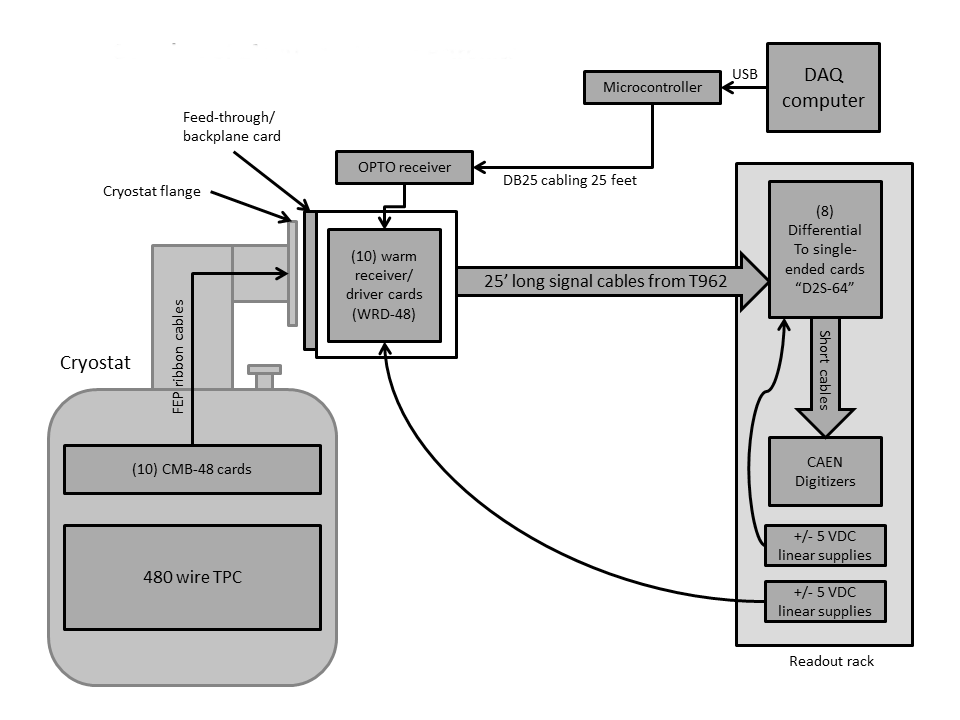
\includegraphics[width=1.0\textwidth]{figures/LArIAT_FE_Electronics.png}
\caption{
Overview of LArIAT Front End electronics. 
} 
\label{pic:FEelectronics}
\end{figure}

The electrical signals on the TPC readout wires are typically quite small, being a direct readout of the ionization of the liquid argon. To achieve a good Signal-to-Noise Ratio (SNR) for such signals, the LArIAT TPC is instrumented with cold amplifiers developed by Brookhaven National Lab (BNL) and mounted directly to the TPC frame inside the liquid argon cryostat. The BNL amplifiers are built as custom Application-Specific Integrated Circuits (ASICs) [ADD reference]. The BNL ASICs adopted in LAriAT are designated as LArASIC, version 4-star.

The LArASICs are mixed signal devices, where the analog amplifier characteristics are controlled by digitally-set parameters. The maximum gain setting of the LArASIC is 25 mV/fc. At this gain a 3.5~fC charge deposition - corresponding to the expected charge arriving at an individual wire from a passing MIP energy deposition - on a readout wire will generate an output with 90~mV amplitude. At the other end of the readout chain, the CAEN V1740 [\textbf{ADD}: CAEN refernece] digitizers have a 12 bit resolution and a maximum input range of 2~VDC, yielding about 0.5~mV LSB. With the analog signal path from LArASIC to the digitizers being designed to provide unity gain, a passing MIP in the TPC is expected to generate a digital signal with amplitude of about 180 ADC counts.  [\textbf{UPDATE}: Dean found gain to be less than unity, add details; what was the measured MIP amplitude?] \textcolor{red}{what is the sampling rate of the board?}

The readout racks containing the signal digitizers are positioned at a distance of $\sim$8~mt from the cryostat and are referenced to a different ground respect to the TPC electronics ground.  The distance minimizes the presence of secondary, tertiary and halo charged particles passing through the digitial electronics.  To prevent problems caused by differing grounds and noise pick-up along the signal transmission line, the single-ended analog signals from the ASICs are transmitted from the cryostat to the readout racks as differential analog pairs, each pair individually shielded.  This is achieved using four types of interconnected cards.  The first type of card in the system is a 48-channel cold motherboard (CMB-48) that mounts directly to the TPC and houses three 16-channel LArASICs per card.  The next card in the signal path is a single cryostat feed through card (FT) that carries the 480 signals, along with power and control lines, across the cryostat boundary.  A set of warm receiver and driver (WRD-48) cards plug directly into the cryostat feed-through and amplify the single-ended TPC signals as differential analog. The differential analog signals are then driven through 8~mt high quality pleated foil cables to a set of differential-to-single-ended (D2S-64) cards, converting the differential signals into single-ended ones, with enough drive capability to allow direct input into an array of CAEN V1740 digitizers.

At the receiving end of the differential path the differential-mode analog signal arrives with common-mode noise cancelled and converted to single-ended analog for the short distance transmission to the CAEN V1740 digitizers.

%%%%%%%%%%%%%%%%%%%%%%%%%%%%%%%%%%%%%%%%%%%%%%%%%%%%%%%%%%%%
\subsection*{Cryostat feed through}
%%%%%%%%%%%%%%%%%%%%%%%%%%%%%%%%%%%%%%%%%%%%%%%%%%%%%%%%%%%%
The feedthrough (FT) card developed for LArIAT is sandwiched between an ASA flange and cap, and sealed with o-rings. A stiff mechanical structure and backplane-style connectors support the FT card and allow for the WRD-48 cards to be plugged directly into it. Such an arrangement facilitates the assembly and potential repair work while reducing the amount of cables and connectors needed.

\begin{figure}[htbp]
 \centering
 \includegraphics[width=0.5\textwidth]{figures/FT_drawings.png}
\caption{
Drawing of LArIAT feed through and Warm Receiver Driver crate. 
} 
\label{pic:FeedthroughElectronics}
\end{figure}

The FT card is built as an 8-layer PCB with dimensions 254~mm $\times$ 432~mm. The outer layers of the card are mostly uninterrupted ground planes to increase noise immunity. The internal traces are built with relatively large 12~mil design rules to enhance manufacturing yield and physical robustness. Signal on adjacent layers are staggered to reduce capacitive cross-talk couplings, and ground fills are provided whenever possible on all copper layers.

Supporting the FT card is a mechanical structure that is rooted on the cryostat flange. The overall assembly of the card, the ten WRD-48 cards, and the WRD card cage is light enough to be safely cantilevered from the cryostat flange. The backplate of the structure is a solid copper sheet which is electrically connected with the cryostat flange though lock washers and also connected to the FT card through 40 conductive standoffs. The copper plate and the cryostat flange are defined as the electrical ground of the TPC readout electronics.

%%%%%%%%%%%%%%%%%%%%%%%%%%%%%%%%%%%%%%%%%%%%%%%%%%%%%%%%%%%%
\subsubsection*{CMB-48 card details}
%%%%%%%%%%%%%%%%%%%%%%%%%%%%%%%%%%%%%%%%%%%%%%%%%%%%%%%%%%%%
Each CMB-48 card holds 3 LArASICs. The card provides electrical connection to the LArIAT TPC wires and mechanical connection to the TPC structure. The CMB-48 board is located inside the cryostat and is thus inaccessible during data-taking periods. The board is designed to minimize the source of electrical noise, the risk of failure due to thermal stress, and the risk of component failure.

%%%%%%%%%%%%%%%%%%%%%%%%%%%%%%%%%%%%%%%%%%%%%%%%%%%%%%%%%%%%
\subsubsection*{WRD-48 card details}
%%%%%%%%%%%%%%%%%%%%%%%%%%%%%%%%%%%%%%%%%%%%%%%%%%%%%%%%%%%%
The WRD-48 cards are designed to be paired one-to-one with the CMB-48 cards inside the cryostat.The WRD-48 cards hold 48 channels of single-ended to differential analog amplifiers to transmit the TPC signals to the distant digitizers. These cards also provide low-noise power regulation, digital signal conditioning, front-panel diagnostic LEDs and voltage monitor ports, and an on-board test-pulse generator. 

%%%%%%%%%%%%%%%%%%%%%%%%%%%%%%%%%%%%%%%%%%%%%%%%%%%%%%%%%%%%
\subsection*{D2S-64 card details}
%%%%%%%%%%%%%%%%%%%%%%%%%%%%%%%%%%%%%%%%%%%%%%%%%%%%%%%%%%%%
The D2S-64 cards convert the differential analog signals from the WRD-48 cards to single-ended signals and drive these signals into the $50 \Omega$ input impedance of the CAEN V1740 digitizers.

The LArIAT data acquisition system is triggered to read out the digitizing buffers by a CAEN V1495 module. The V1495 is a powerful, easily configurable coincidence module featuring a user-programmable FPGA.  Sixteen logical inputs (upgraded to 32 in Run-III) are sampled on a 10~ns clock, checking for matches to any of the sixteen user-defined patterns in the trigger menu.  If a given trigger pattern is satisfied for two consecutive clock ticks, that pattern fires. 

NIM-standard logic pulse inputs to the trigger decision come from any of the instruments in the experiment, in principle; trigger inputs are derived from beam instruments, from the cosmic ray taggers, and from the cryostat's scintillation detectors. LArIAT takes full advantage of the trigger card's great flexibility.  As conditions change and innovations are gradually made to LArIAT's data-taking process, improvements are made to the trigger input designs and the combinations of inputs which define trigger patterns for the V1495.  The configuration of the trigger inputs is automatically logged in a database at the start of each run as part of the DAQ configuration, along with the rest of the XML configuration file for the V1495.

\subsubsection{Inputs to the Trigger System}

Two primary inputs to the trigger card are from the time of flight (see Sec.~\ref{sec:TOF}) and the wire chamber (see Sec.~\ref{sec:MWPC}) systems in the tertiary beamline.  Coincidence of activity in both of these systems strongly suggests that a charged particle has made the journey down the tertiary beam line from the copper target to the LArTPC in the cryostat, and that we will have a measure of its momentum and its velocity. PMT pulses from the time of flight system each pass through a 
%FIXME WHAT MODEL linear fanout?
linear fan-out, one output of which is threshold discriminated by a
%FIXME WHAT MODEL
discriminator to produce a NIM logic pulse for use in trigger logic.  On each of the upstream or downstream TOF paddles, we form a coincidence to within 20~ns of pulses from all the PMTs observing that same block of scintillator.  The upstream paddle coincidence signal is delayed 20~ns to allow any approximately lightspeed particles to travel 6.5~m to the downstream paddle.  The same upstream paddle coincidence signal is also widened to 100~ns to allow for slow-traveling (high-mass) particles.  Coincidences of these upstream and downstream TOF trigger input signals can be made in the V1495 trigger card.

Each wire chamber is read out by four multi-hit TDCs (time to digital converters), with sixty-four wires per TDC and two TDCs per plane (one horizontal and one vertical).  The TDCs each provide a logical ``fast'' OR of their inputs, indicating that one or more of their sixty-four wires went over the settable threshold.  Using NIM logic units, the OR of the horizontal wires and the OR of the vertical wires are input to a coincidence unit for each wire chamber, providing a single logical pulse for each of the four wire chambers, indicating that at least one horizontal wire and one vertical wire saw significant signal.  The single culminating logical pulses from each of the four wire chambers make up the first four inputs to the V1495 trigger card.  Within the user-programmable FPGA, the V1495 looks for the coincidence within 20~ns of at least three of these four specially-treated logical inputs.

Another primary input to the trigger card is from the cosmic towers (see Section~\ref{sec:CosmicRayPaddle}). To capture cosmic ray events in which a minimally ionizing cosmic ray muon crossed the TPC along the body diagonal, NIM modules form the logical coincidences from the two cosmic towers, one upper and one lower paddle assembly, in each combination.  The OR of these is provided as an input to the V1495. 

Three important logic pulses are derived from the timing of the beam.  These include a pulse in a brief window before the beam, a pulse indicating that the beam is on, and a pulse which defines the beam-free period which may be used for collecting cosmic-ray events.  An adjustable pulser is a fourth trigger input which does not depend on any particular activity in the experiment hall,  useful for collecting background events with zero bias. 

The PMTs observing liquid argon scintillation light (see Section \ref{sec:PhotonSystem}) produce pulses which form the foundation of several interesting trigger inputs.  Thresholding a copy of each PMT pulse (after amplification), and requiring a coincidence of pulses within $\sim$20~ns, creates simple trigger inputs indicating ionizing radiation was produced in the TPC.  This scintillation logic pulse is used to initiate a gate which spans the length of the TPC drift time, creating a logic signal which is remains ``on'' while significant drift charge may still be present in the TPC.  In addition, requiring a delayed coincidence of two subsequent scintillation logic pulses, separated by a variable length of time ranging from 300~ns to 7~$\mu$s, is used to create a trigger input to select events where a cosmic muon stops and decays to a Michel electron in the TPC.  A few different versions of this light-based trigger were implemented throughout the course of LArIAT's run time to allow reconstruction and calorimetric studies of Michel electrons. Figure~\ref{michel_logic} shows a schematic diagram of the logic comprising the Michel electron trigger. 

\begin{figure}
\includegraphics[width=\textwidth]{figures/trigger_michellogic.png}
\caption{\label{michel_logic}A schematic diagram of the trigger logic used to select Michel electron events during the cosmic readout window of the LArIAT supercycle.  The two PMT signals refer to the Hamamatsu (``HMM'') and ETL PMTs described in Section~\ref{sec:PhotonSystem}.  For some data-taking periods in Run-II, un-amplified pulses were discriminated at 180 mV to act as a veto on events that may saturate the dynamic range of the V1751 digitizer.  The discriminator thresholds used on the amplified (x10) PMT signal copies (\emph{ThA}, \emph{ThB}) as well as the Gate Delay period, were adjusted between run periods while experimenting with different configurations.}
\end{figure}

Further trigger inputs come from the beam line instrumentation behind the LArTPC cryostat, the PMTs of the Punch-Through scintillator paddles and those of the scintillator paddles instrumenting the Muon Range Stack.  The PMT pulses of all four of the broad-faced Punch Through paddles are discriminated to form logic pulses.  A single logic pulse is formed from these, indicating activity in at least two overlapping paddles at the rear of cryostat, before the steel block of the range stack.  PMT pulses from the Muon Range Stack are amplified and threshold discriminated.  These MuRS paddle pulses are then combined as in the Punch Through, creating single-bit indicators for each of the four instrumented layers that at least one pair of overlapping scintillator paddles sent signals within a 20~ns coincidence window.

\subsubsection{Trigger Decision and Issuance}

The V1495 may be configured to have up to sixteen trigger patterns and sixteen veto patterns, based on the trigger input signals.  A trigger pattern is defined as the AND of one or more defined inputs, and may include the NOT of the AND of further inputs.  Veto patterns are independently defined in the same way, but they have a very different effect.  When any of the trigger patterns fire, a ``fast trigger'' signal is issued and an adjustable countdown is initiated.  If the countdown completes without a veto pattern firing, the ``slow trigger'' signal is also issued and on a distinct hardware channel. Otherwise, if a veto pattern fires during the countdown, the slow trigger signal is vetoed.  

The fast trigger signal prompts readout of all the `short' data buffers, which include the V1751 modules, the V1495 itself, and the MWPC controller.  The V1751 buffers typically contain digitized PMT signals from the time of flight and cryogenic light collection detectors. Readout of the TPC wire signals, which are much longer and more numerous, is only prompted at the issuance of the slow trigger.

In addition to the drift electrons, LArIAT also collects liquid argon scintillation photons.  This is achieved using several cryogenic photodetectors held in place by a PEEK support structure which screws into a side access flange as shown in Figure~\ref{lightsys_pmts}.  Two PMTs, a 3-inch diameter Hamamatsu R-11065 and 2-inch diameter ETL D757KFL~\cite{lightsys-pmttests}, contribute to most of the system's light collection capacity.  During Run-I and Run-II, several silicon photomultiplier (SiPM) arrays were also included as part of the photon detection system.  These SiPMs consisted of two Hamamatsu S11828-3344M 4x4 arrays (each with 12x12mm$^2$ total active area) as well as one single-channel SensL MicroFB-60035 (6x6mm$^2$ active area) on custom preamplifier readout boards which were mounted along the edges of the PMT holder.  The windows of all devices are held parallel to the wireplanes with approximately 5~cm of clearance.

%------------------------------------------
\begin{figure}
\centering
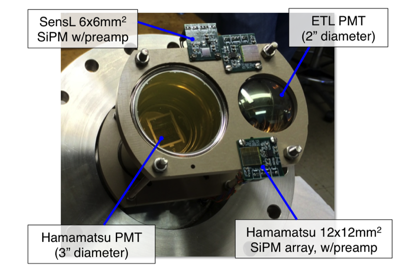
\includegraphics[height=2.2in]{figures/lightsys_pmts.png}
\hspace{1cm}
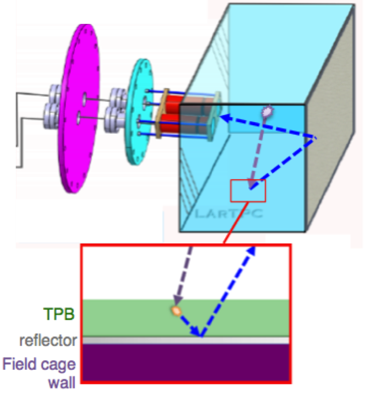
\includegraphics[height=2.2in]{figures/lightsys_wls.png}
\caption{LArIAT's photodetector system for observing LAr scintillation light inside the TPC (left), and a simplified schematic of VUV light being wavelength-shifting along the TPB-coated reflecting foils (right).}
\label{lightsys_pmts}
\end{figure}
\begin{figure}
\centering
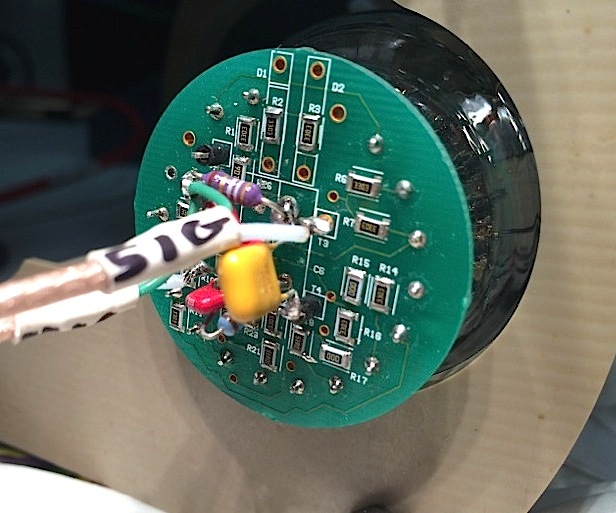
\includegraphics[height=0.25\textheight]{figures/lightsys_etlbase.jpeg}
\hspace{0.5cm}
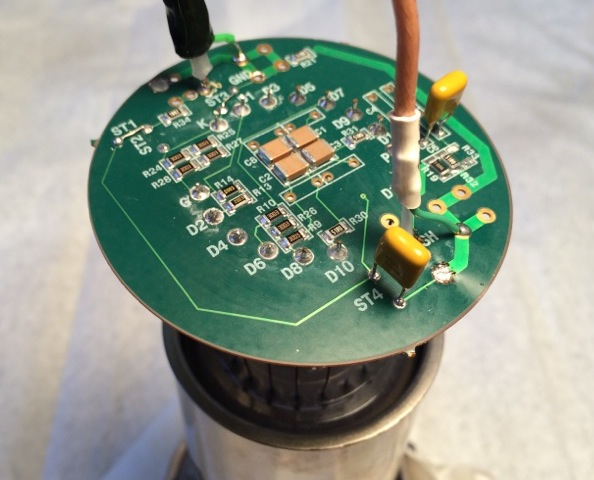
\includegraphics[height=0.25\textheight]{figures/lightsys_hmmbase.jpg}
\caption{\label{voltagedividers}Photos of the voltage divider bases for the ETL PMT (left) and the Hamamatsu PMT (right) used in Run-II.  The cable connections to the bases seen here were used for powering and testing prior to installation.  The yellow through-hole signal coupling capacitors seen on both bases are 18~nF (X7R) and are rated to 2~kV.}
\end{figure}
%------------------------------------------


Liquid argon scintillation light is produced in the vacuum-ultraviolet (VUV) range and must be shifted to visible before it can be detected by most photosensors.  This wavelength-shifting occurs within a thin layer of tetraphenyl-butadiene (TPB) which coats highly-reflective VIKUITY dielectric substrate foils lining four walls of TPC.  A photo of these foils mounted inside the TPC is shown in Figure~\ref{lightsys_foils}.  A VUV photon interacts with the TPB to induce emission of one or more visible photons which are then emitted or reflected back into the active volume, increasing the probability of their detection by the photosystem~\cite{lightsys-szelc}. This technique also improves light yield uniformity across the TPC's active volume, a feature relevant to light-augmented calorimetry.

%------------------------------------------
\begin{figure}
\centering
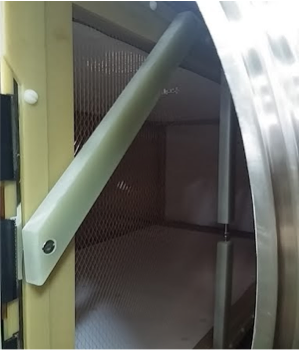
\includegraphics[scale=1.3]{figures/lightsys_foils.png}
\caption{\label{lightsys_foils}The TPB-coated reflector foils mounted to the TPC field cage walls as viewed through the front cryostat opening. {\textcolor{red}{Better pictures needed.}}}
\end{figure}
%------------------------------------------


A TPB coating\footnote{The TPB coating was made using a solution of 100~mL toluene, 2~g polystyrene, and 800~mg of TPB prior to Run-II. The coating was re-applied to the ETL midway through Run-II using the same solution but with less TPB (600~mg).} was added to the windows of the ETL PMT and SensL SiPM prior to Run-II and reapplied about midway through the run.  This allowed some of the VUV scintillation light to down-convert directly at their faces instead of at the coated reflector foils, rendering the photodetectors directionally sensitive to this light emanating from the point of energy deposition.  These coatings were removed prior to Run-III.

For Run-I, the voltage dividers for the PMTs were configured for negative bias with a DC-coupled anode, and were switched to positive bias mode (AC-coupled anode with grounded photocathode) for Run-II to minimize induced noise on wires near the charged photocathodes and outer PMT chasis.  To configure each base for positive polarity before the start of Run-II, 18 nF (X7R) capacitors rated to 2kV were soldered onto the circuits to couple each PMT's anode to the outgoing signal line.  At liquid argon temperature and PMT operating voltages, these capacitances reduce to $\sim$1/3 of their nominal value~\cite{lightsys-capacitors,lightsys-ubsplitting}.

For Run-III, a prototype ARAPUCA~\cite{lightsys-arapuca} detector was installed, replacing the SiPM boards. The main purpose of the prototype is research and development of new alternatives for photosensors for liquid argon-based detectors.
The central concept of ARAPUCA is to capture photons within a box with highly reflective internal surfaces (reflectivity~>~98~\% ), resulting in high photon detection efficiency even for limited active coverage, which is defined as the total area of photosensors viewing the internal volume. The key to the ARAPUCA's photon-trapping mechanism is the use of dichroic short-pass optical filters which are highly transparent to wavelengths below a particular cutoff and highly reflective above it. The filter is externally coated by a wavelength-shifting (WLS) film. The WLS film on the outer side of the filter converts the VUV scintillation light from the liquid argon to a wavelength below the cutoff, so the filter is transparent to the incident photons, allowing them to enter into the box. A second WLS coating covers the inner side of the filter or optionally the internal walls of the box. The internal WLS layer enables a photon to convert a second time to a wavelength greater than the cutoff condition for which the filter is highly reflective, trapping the photons inside the box. The interior of the ARAPUCA is viewed by light sensors which capture the trapped photons after few reflections.
%covered by one or more SiPMs. The number of SiPMs can be increased and read out using an active ganging circuit. Figure \ref{arapuca-principle} illustrates the working principle of the device.

The prototype ARAPUCA device installed in LArIAT, shown in Figure~\ref{fig:arapuca_photo}, is 4.5$\times$5.5 cm$^2$, with a total exposed filter area of 3.5$\times$4.5 cm$^2$.  The WLS film on the outer surface of the filter is P-Terphenyl ($\lambda \sim  350$~nm), while the inner surface is coated in TPB ($\lambda \sim 430$ nm). It is equipped with a single SensL MicroFC 60035 SiPM biased at +24~V in liquid argon.  Its signals are sent through a commercial preamplifier before being sent to the DAQ.

%------------------------------------------
\begin{figure}
\centering
\includegraphics[height=5cm]{figures/lightsys_arapuca2.jpg}
\hspace{0.5cm}
\includegraphics[height=5cm]{figures/lightsys_arapucaPmts.jpg}
\caption{The prototype ARAPUCA device without its dichroic filter (left) as well as mounted to the PMT support structure after the installation of the filter (right).}
\label{fig:arapuca_photo}

\end{figure}
%------------------------------------------

\subsection*{Signal Digitization}

Signals from all photodetectors are routed from the side-flange of the cryostat to NIM fan-outs to provide the 50-Ohm termination needed to minimize reflections along the cables. Copies of the PMT signals are made to aid in several light-based triggers, and copies of all signals are then recored into data using CAEN V1751 digitizer boards with 1~GHz sampling rate.

%------------------------------------------
\begin{figure}
\centering
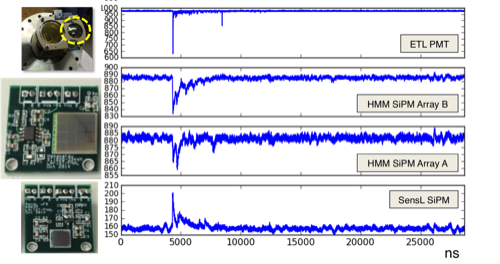
\includegraphics[width=0.8\textwidth]{figures/lightsys_signals.png}
\caption{Some example signals, in ADC units, from LArIAT photodetectors for a triggered cosmic Michel electron event.}
\label{lightsys_signals}
\end{figure}
\begin{figure}
\centering
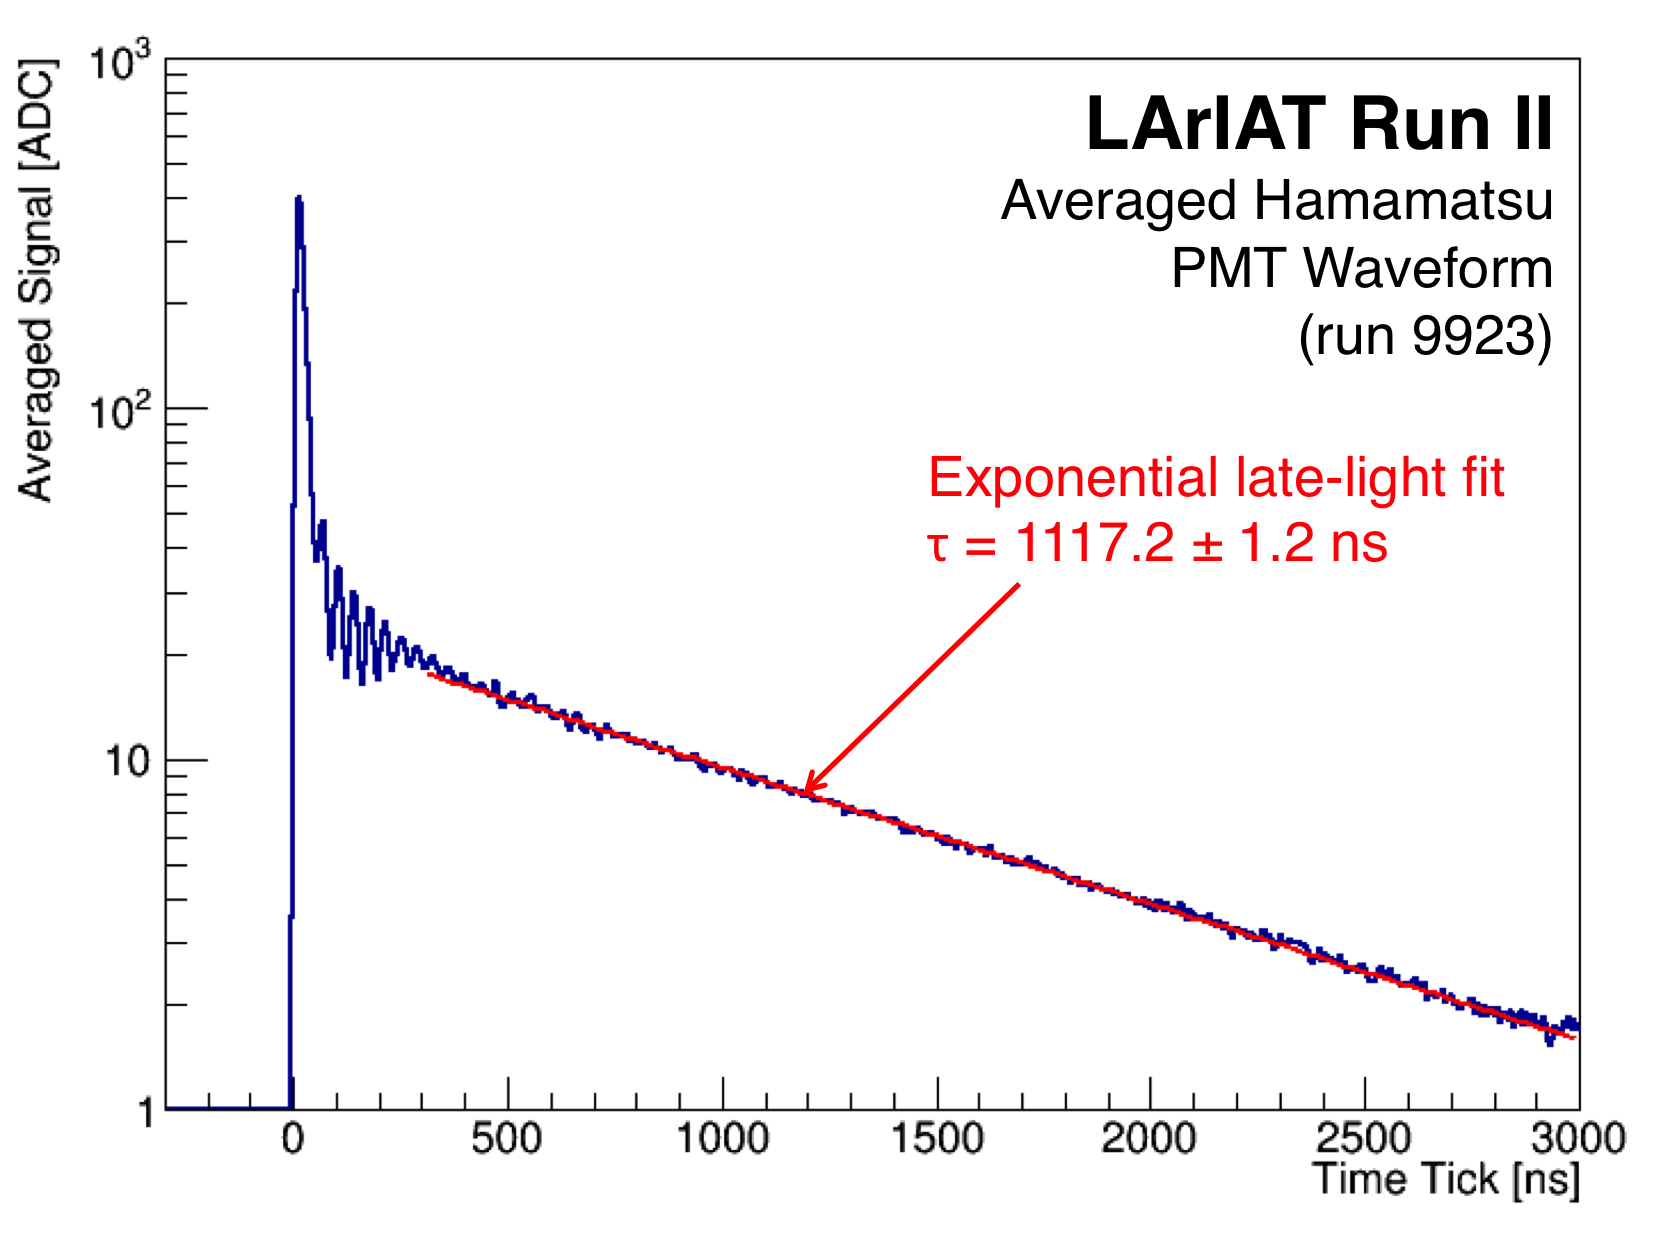
\includegraphics[width=0.6\textwidth]{figures/lightsys_avewfm_hmm.png}
\caption{\label{wfm_hmmpmt}An example of an averaged inverted waveform of the Hamamatsu PMT after event-by-event noise removal and overshoot correction.  Data was taken from a small subset of events from Run-II.  In this example, a falling exponential is fit to the signal region from 300~ns to 3~$\mu$s following the onset of the pulse to extract the late-light component lifetime $\tau$ = 1117~ns.}
\end{figure}
%------------------------------------------

\subsection*{Nitrogen Contamination Measurement Using Light}

The light detection system can also be used to derive information about the nitrogen (N2) contamination in liquid argon. The influence of N2 on liquid argon scintillation light emission has been observed in the WArP experiment~\cite{WARP-nitrogen}. With a higher N2 concentration, the observed decay time of the liquid argon slow component decreases significantly, from over 1~$\mu$s to hundreds of nanoseconds. In this measurement, waveforms recorded by the ETL PMT in Run-I, selected to cover periods of varying N2 concentrations (as measured by the external sensor in Figure~\ref{light_nitro}), were analyzed. An exponential fit was performed to estimate the decay time of the slow light component. Results, shown in Figure~\ref{light_nitro}, were compared with the model from the WArP paper~\cite{WARP-nitrogen}.

%------------------------------------------
\begin{figure}
\includegraphics[height=0.2\textheight]{figures/nitrosensor.jpeg}
\hspace{0.5cm}
\includegraphics[height=0.2\textheight]{figures/nitro_qt.jpeg}
\label{light_nitro}
\caption{Concentration of N2 in LArIAT as measured by an external sensor in Run-I (left), and results of fitting exponential models to waveforms recorded by the ETL PMT compared with the model from WArP~\cite{WARP-nitrogen} (red line).}
\end{figure}
%------------------------------------------
